\NewChapter{个人摄影作品}

除了游戏和游戏设计之外,我最大的爱好便是摄影和音乐。在学习摄影和音乐的过程中,跨界的思维常常给我带来不一样的启发。色彩、构图、组成、旋律、节奏,这些艺术领域相通的元素总能带给我全新的视角.

以下是节选的一些摄影作品。大部分摄自尼康Z72和宾得K2。

\begin{figure}[H]
  \centering

  \subfigure[大雪]{
    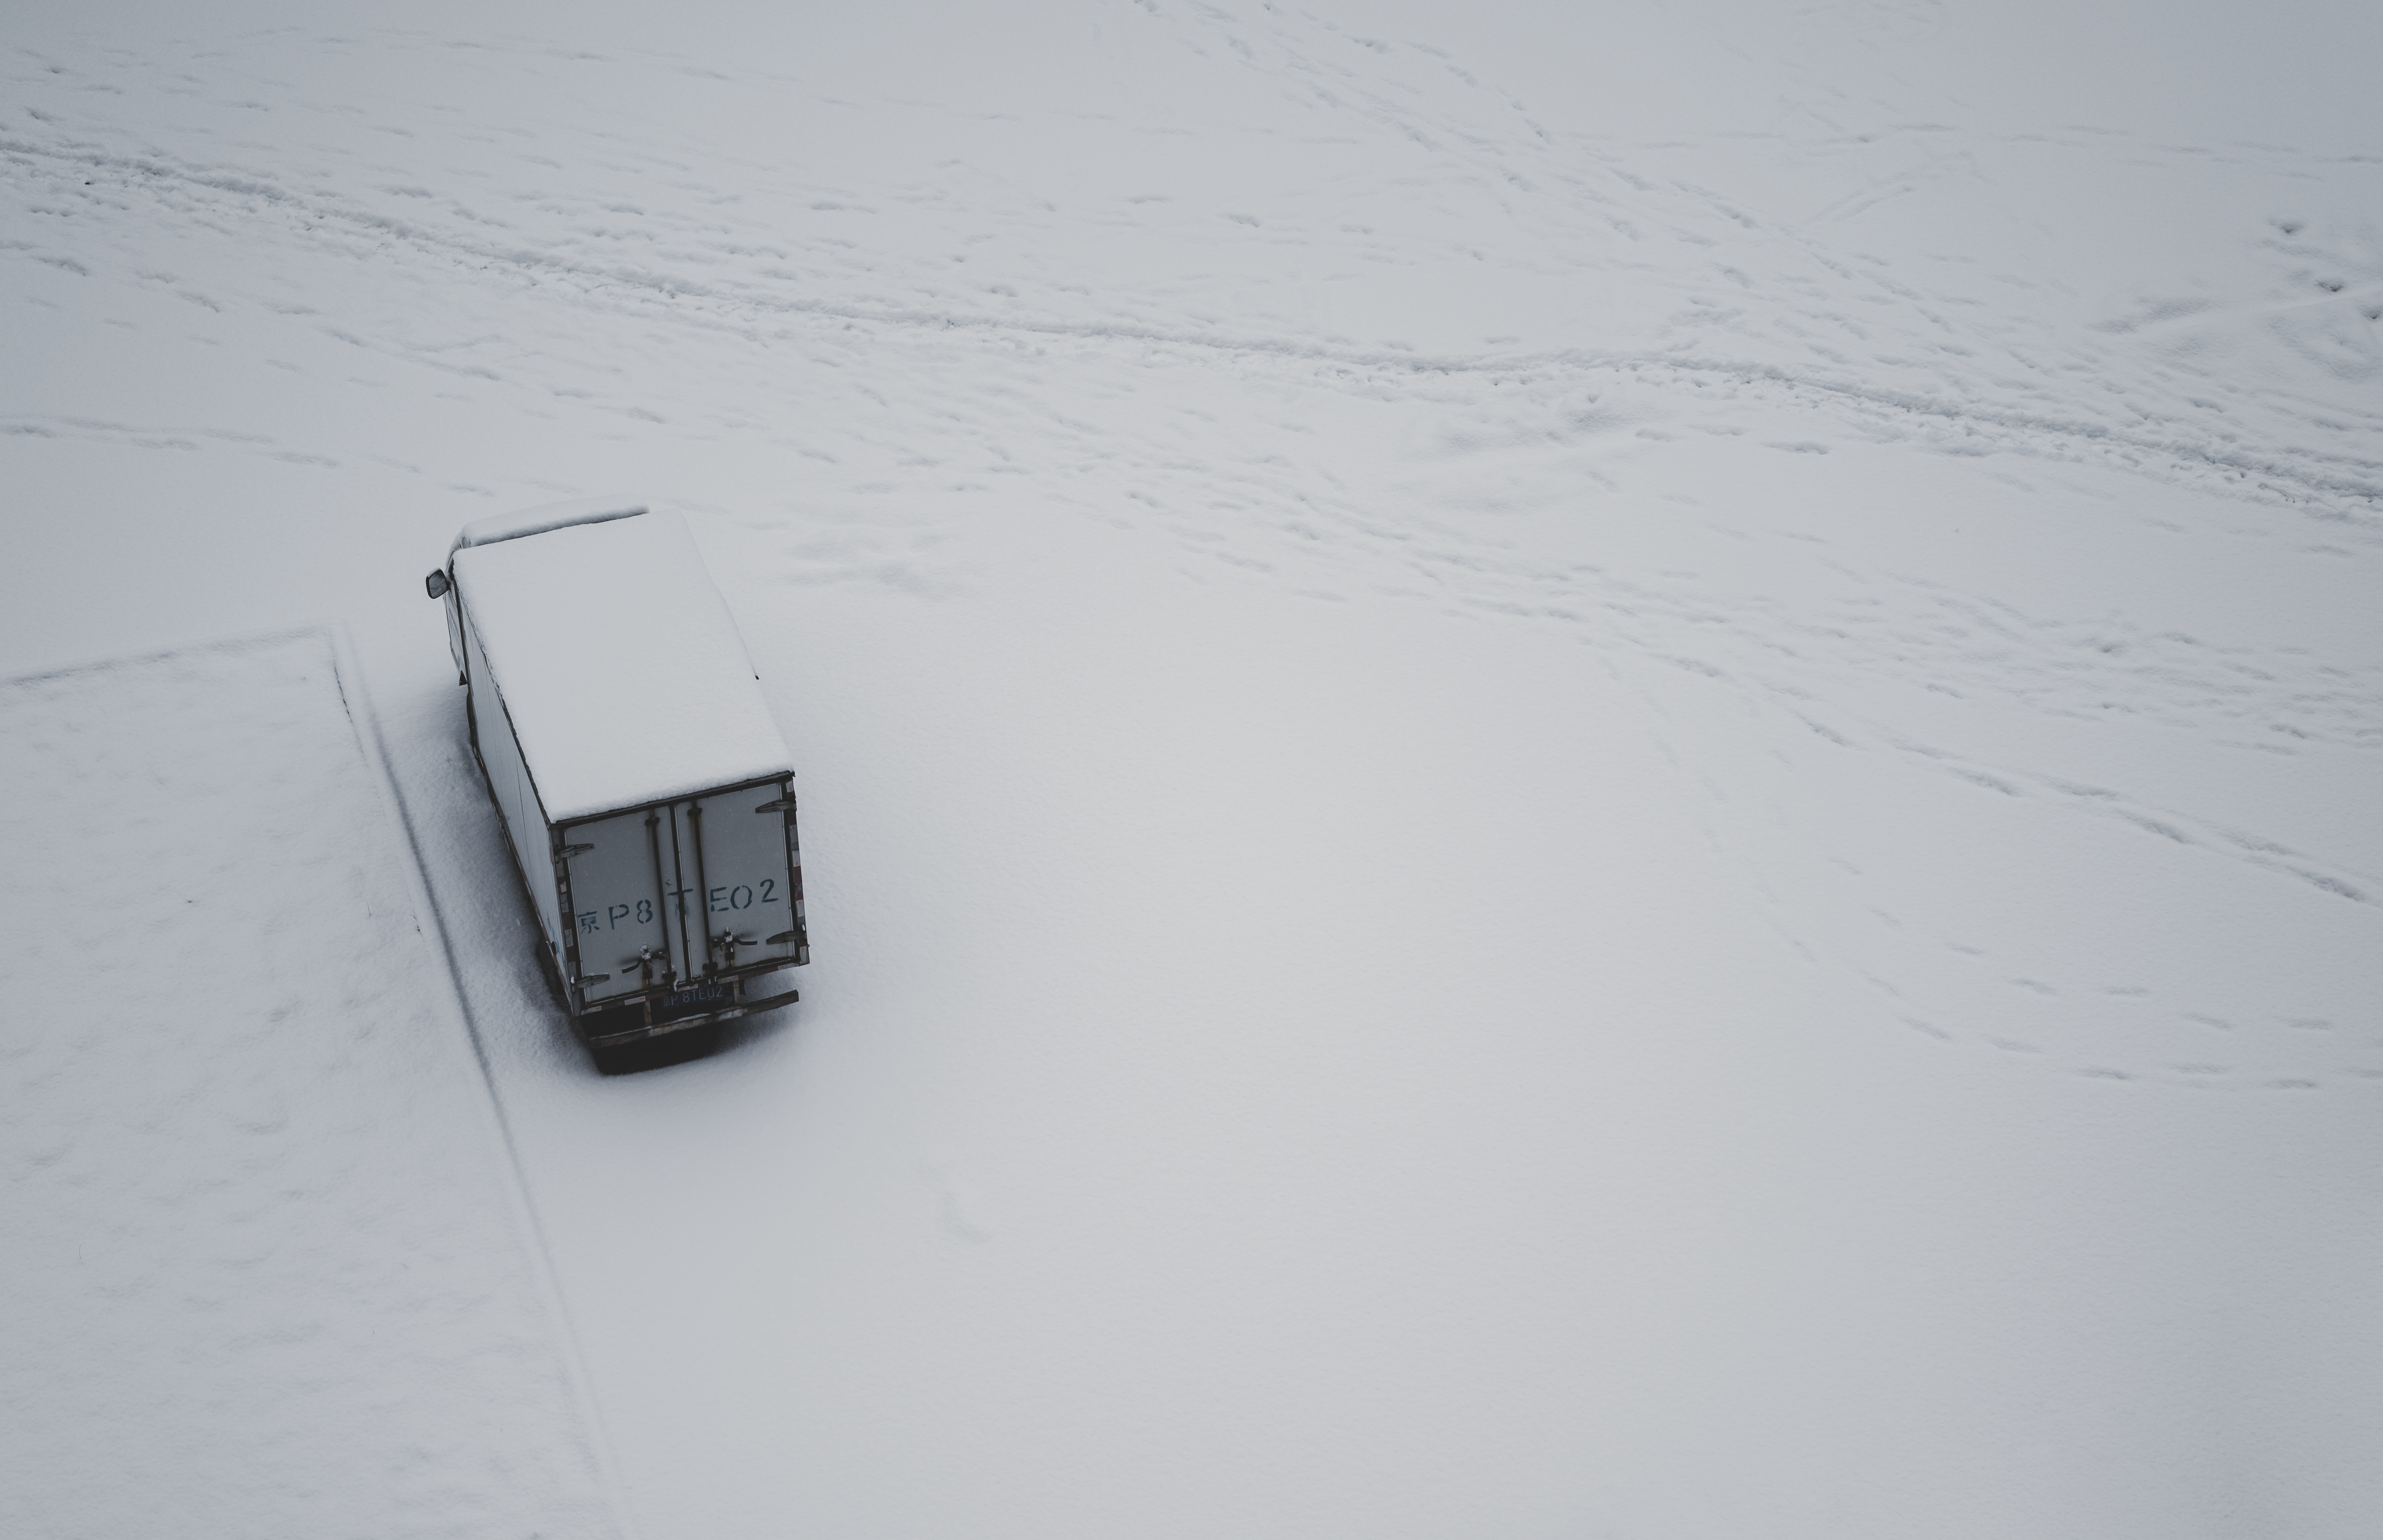
\includegraphics[width=0.9\textwidth]{Images/Photos/h3.png}}
  
  % \subfigure[童年]{
  %   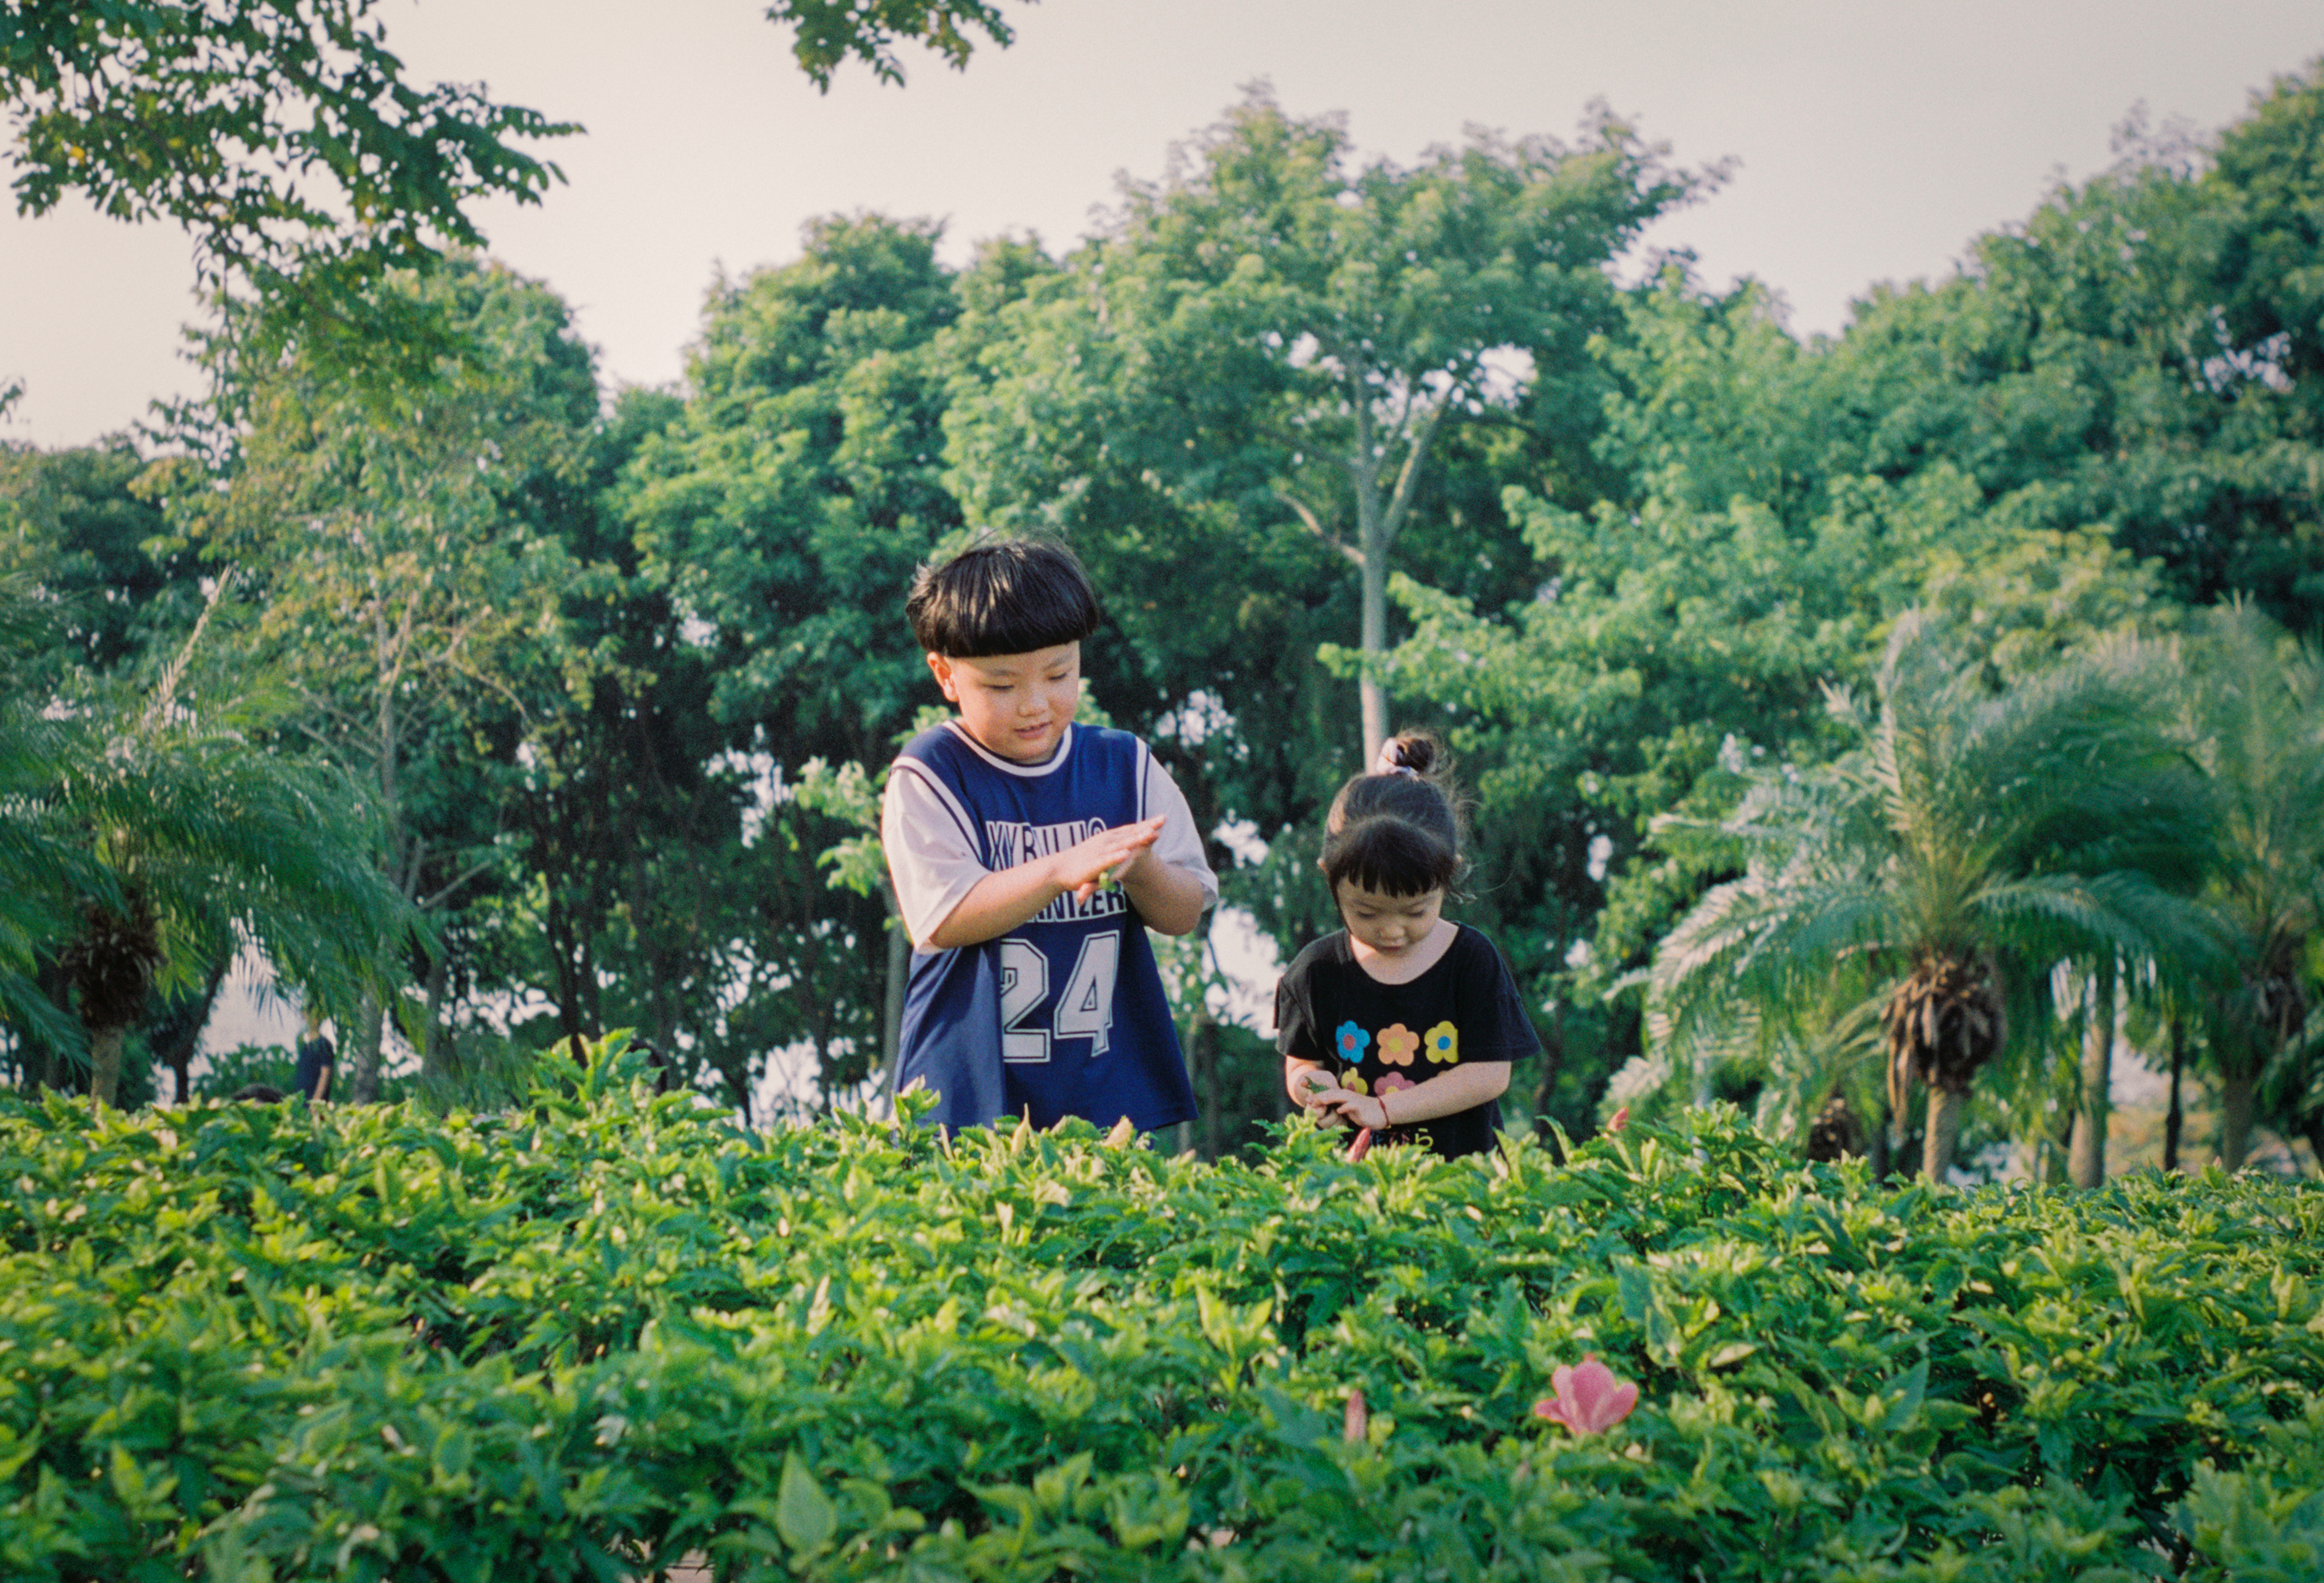
\includegraphics[width=0.45\textwidth]{Images/Photos/h1.jpg}}
  % \subfigure[车站]{
  %   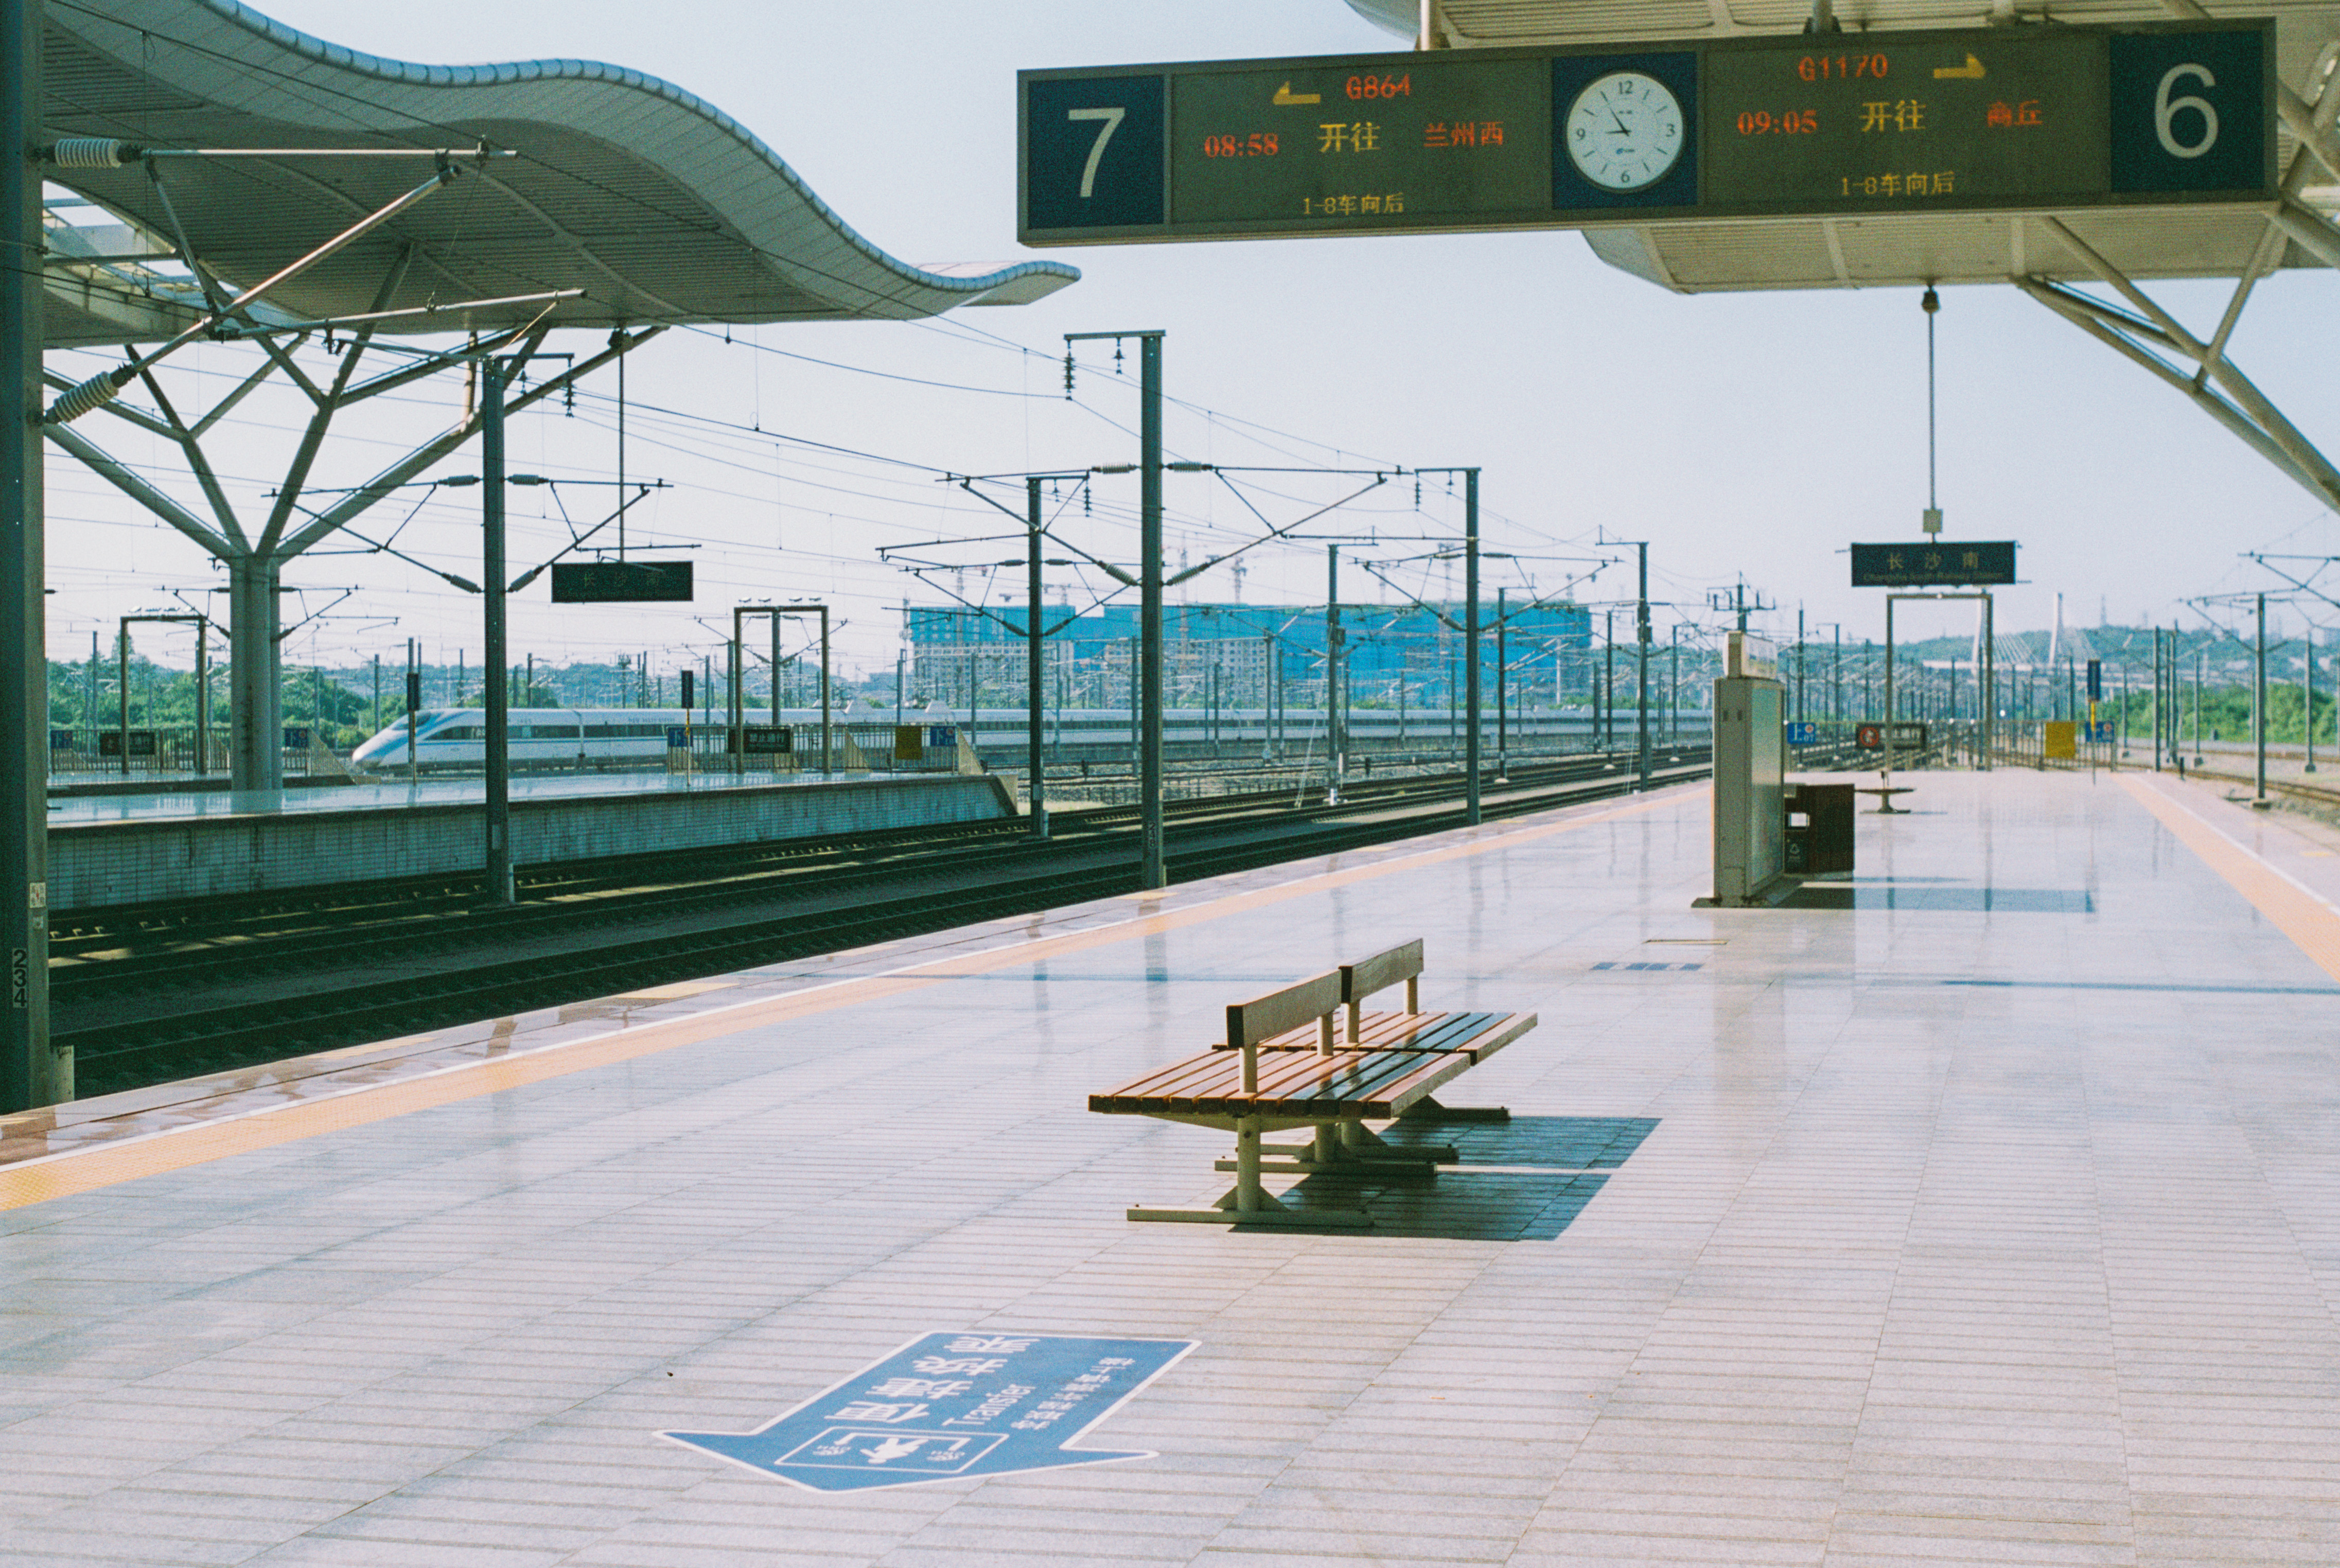
\includegraphics[width=0.45\textwidth]{Images/Photos/h2.jpg}}

  % \subfigure[草甸]{
  %   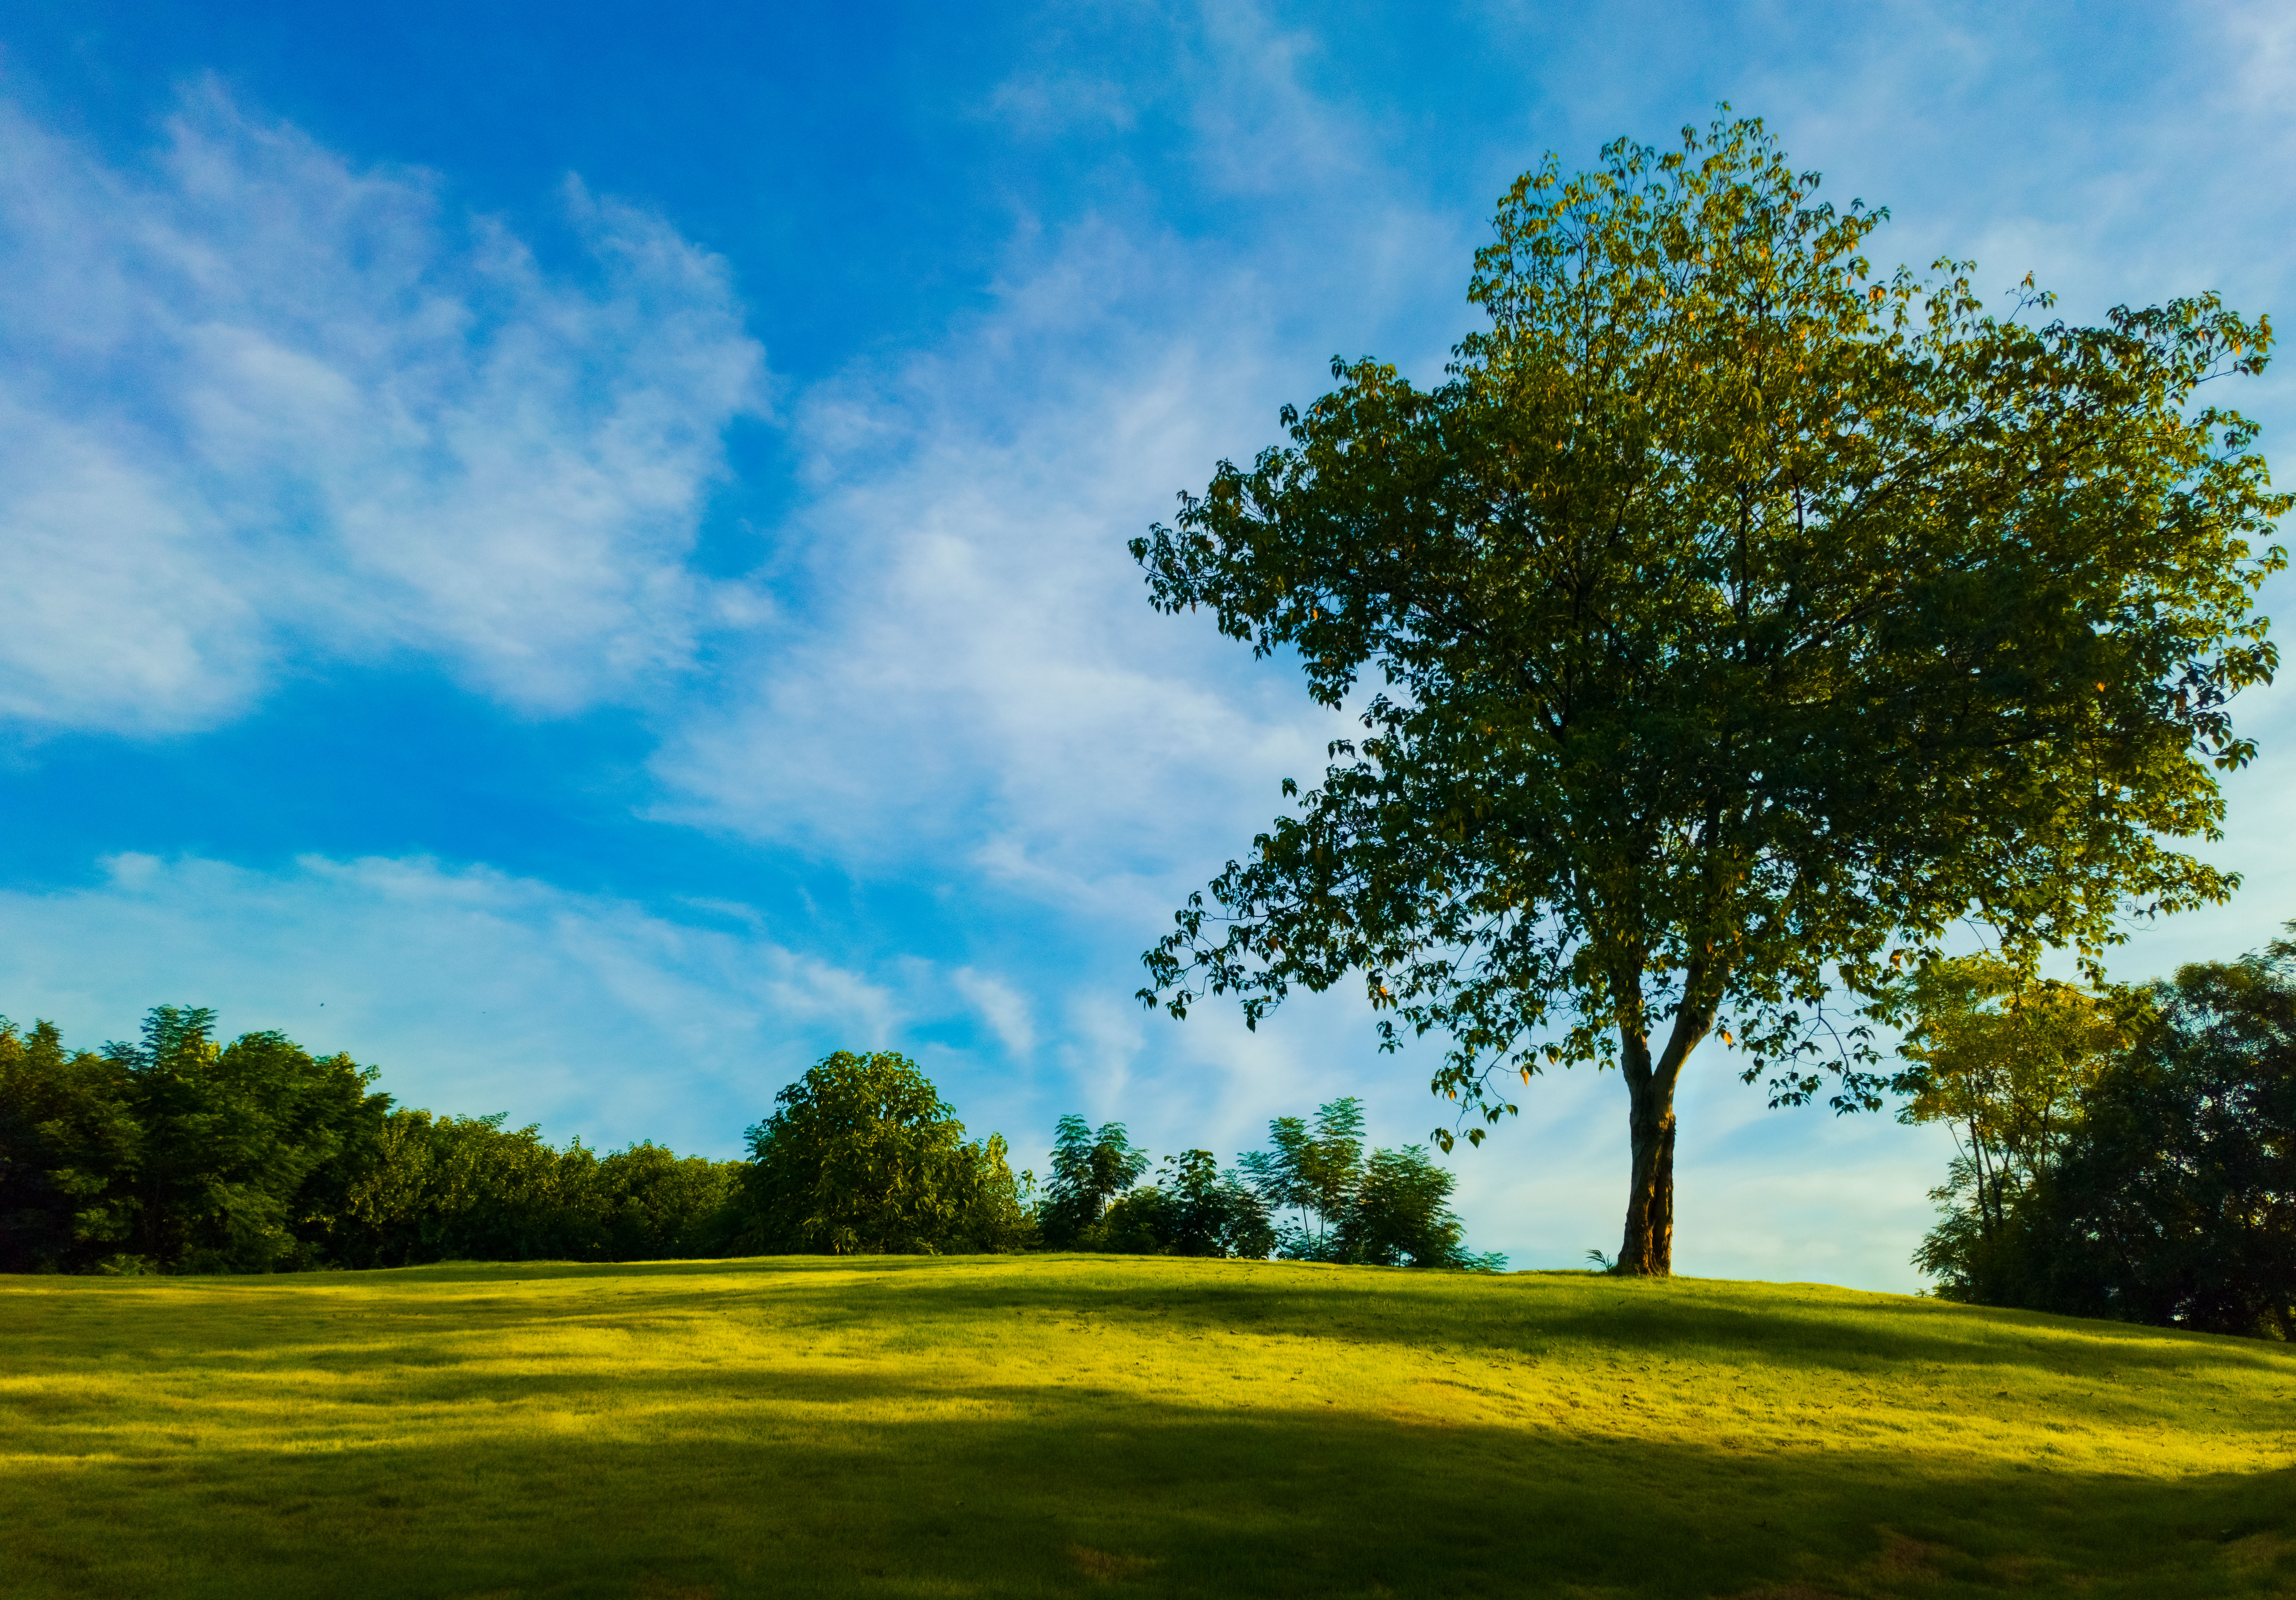
\includegraphics[width=0.45\textwidth]{Images/Photos/h4.jpg}}
    \subfigure[车站]{
    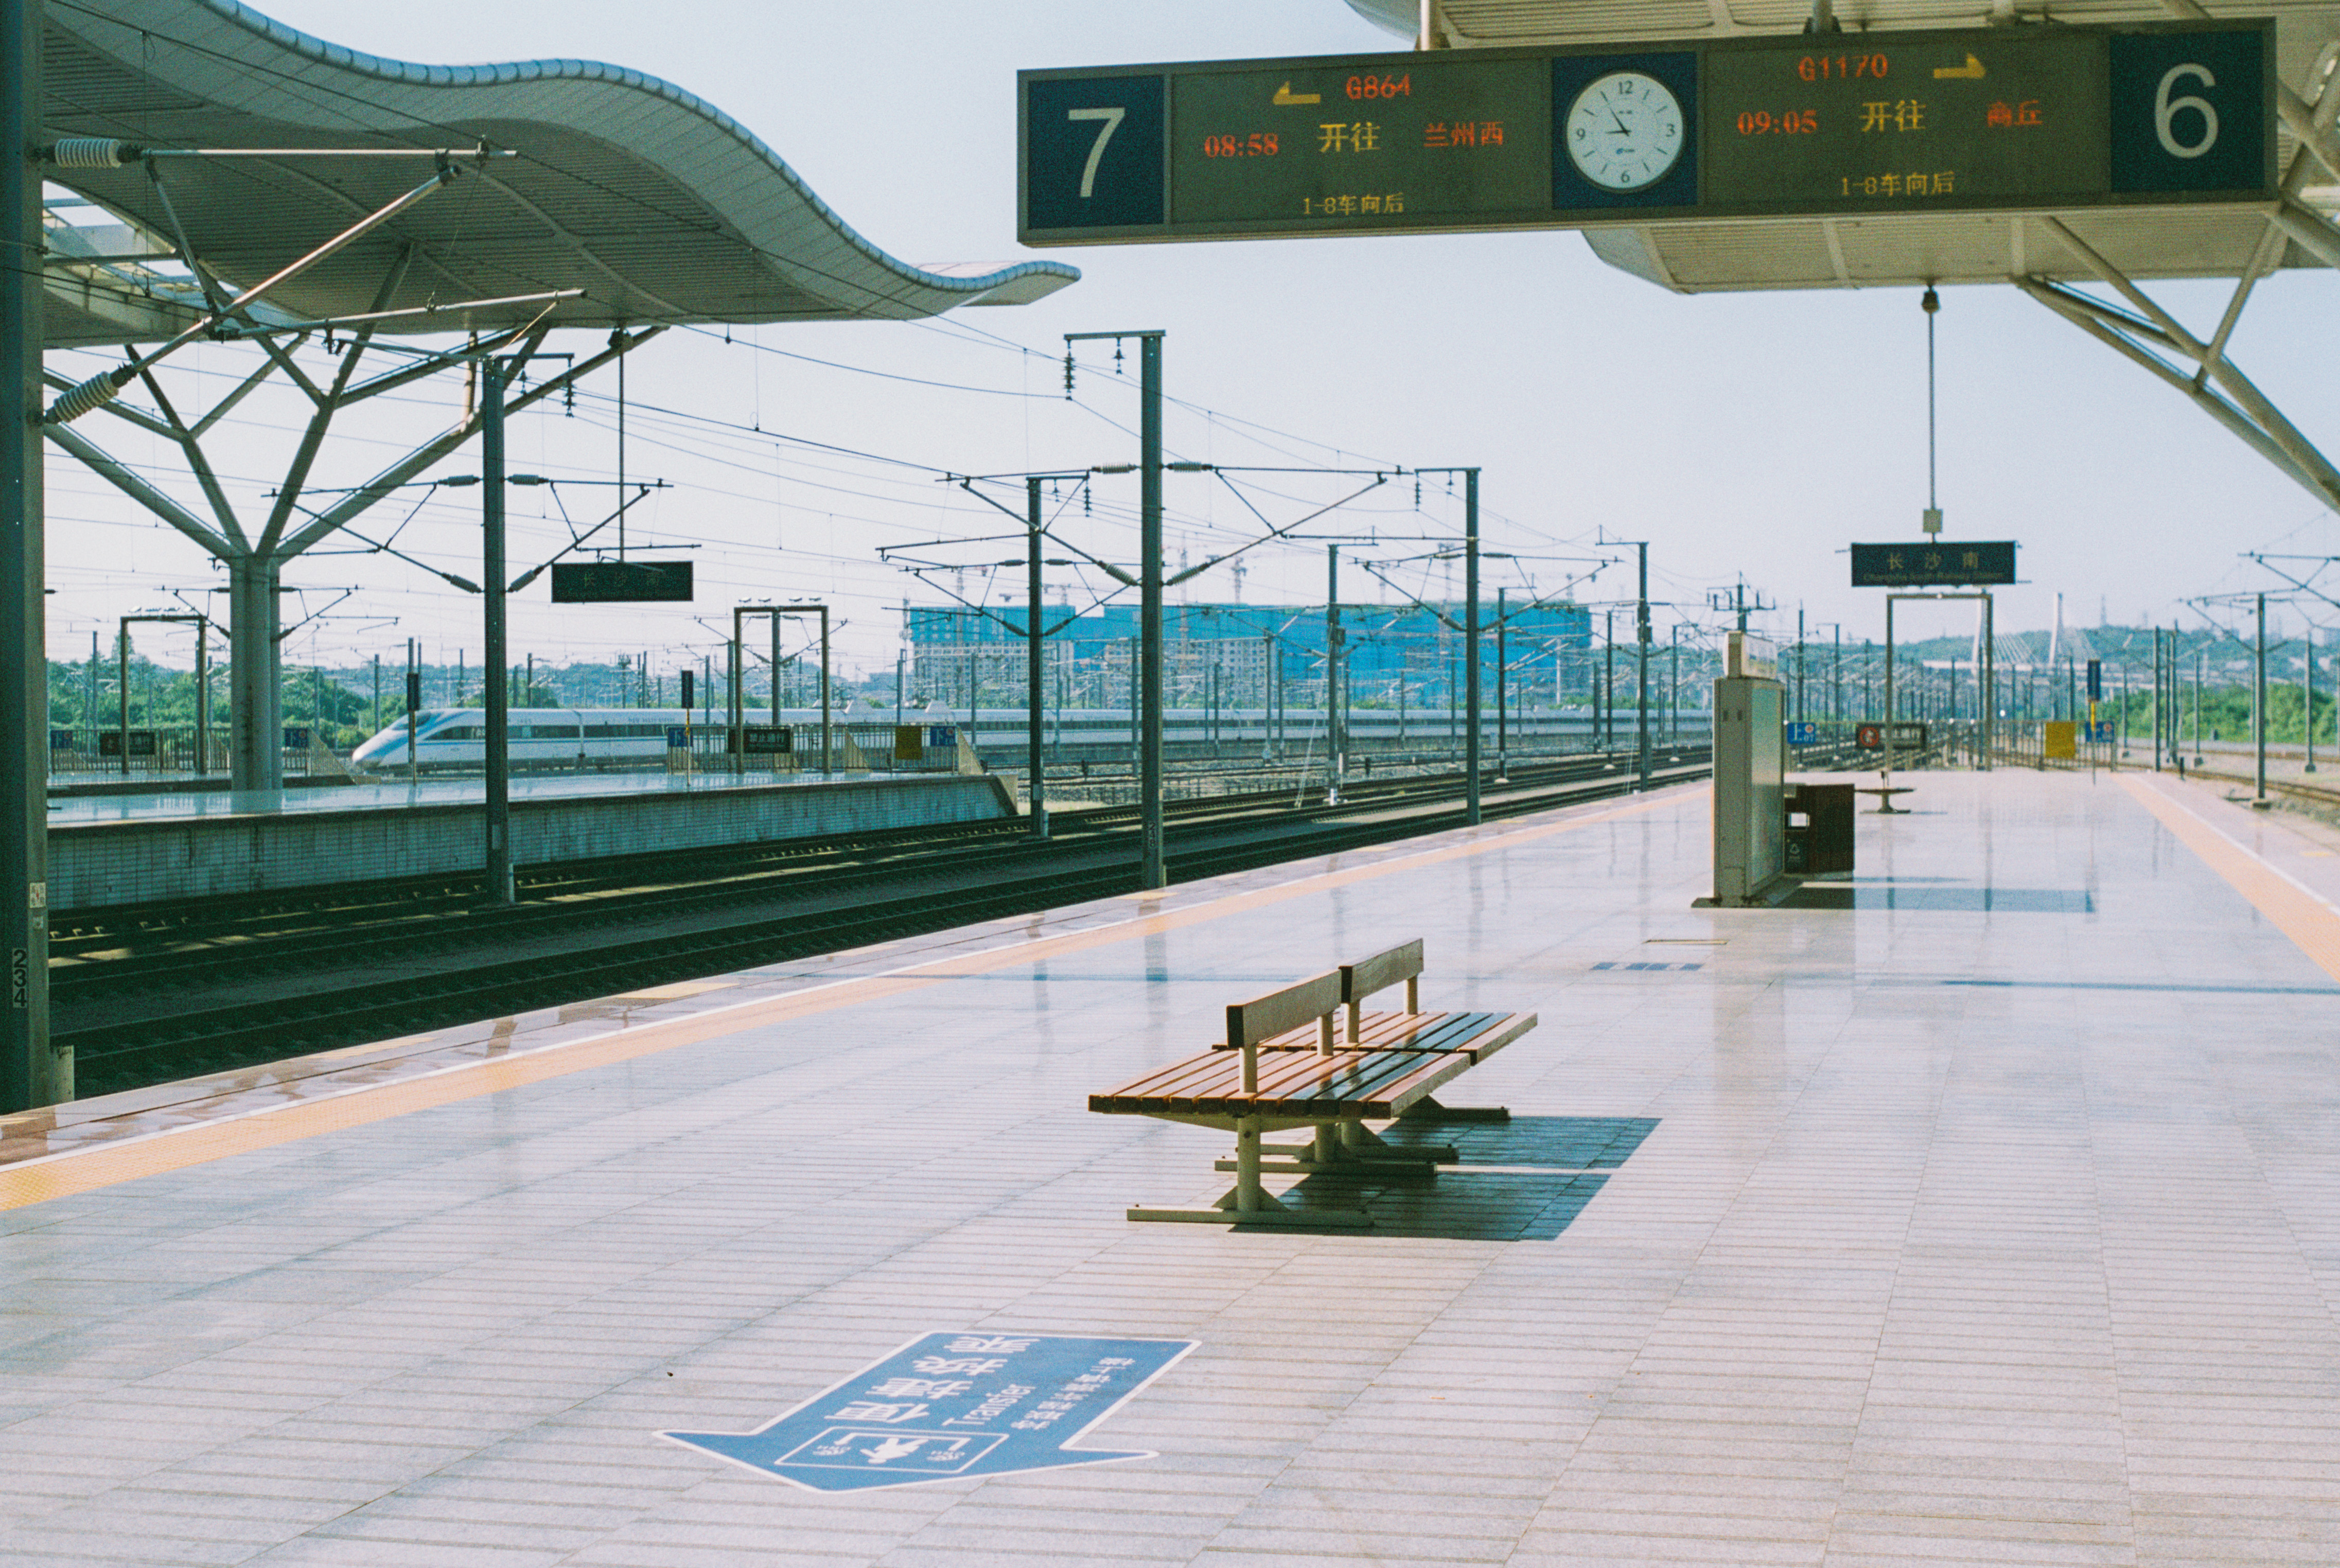
\includegraphics[width=0.45\textwidth]{Images/Photos/h2.jpg}}
    \subfigure[船藻]{
    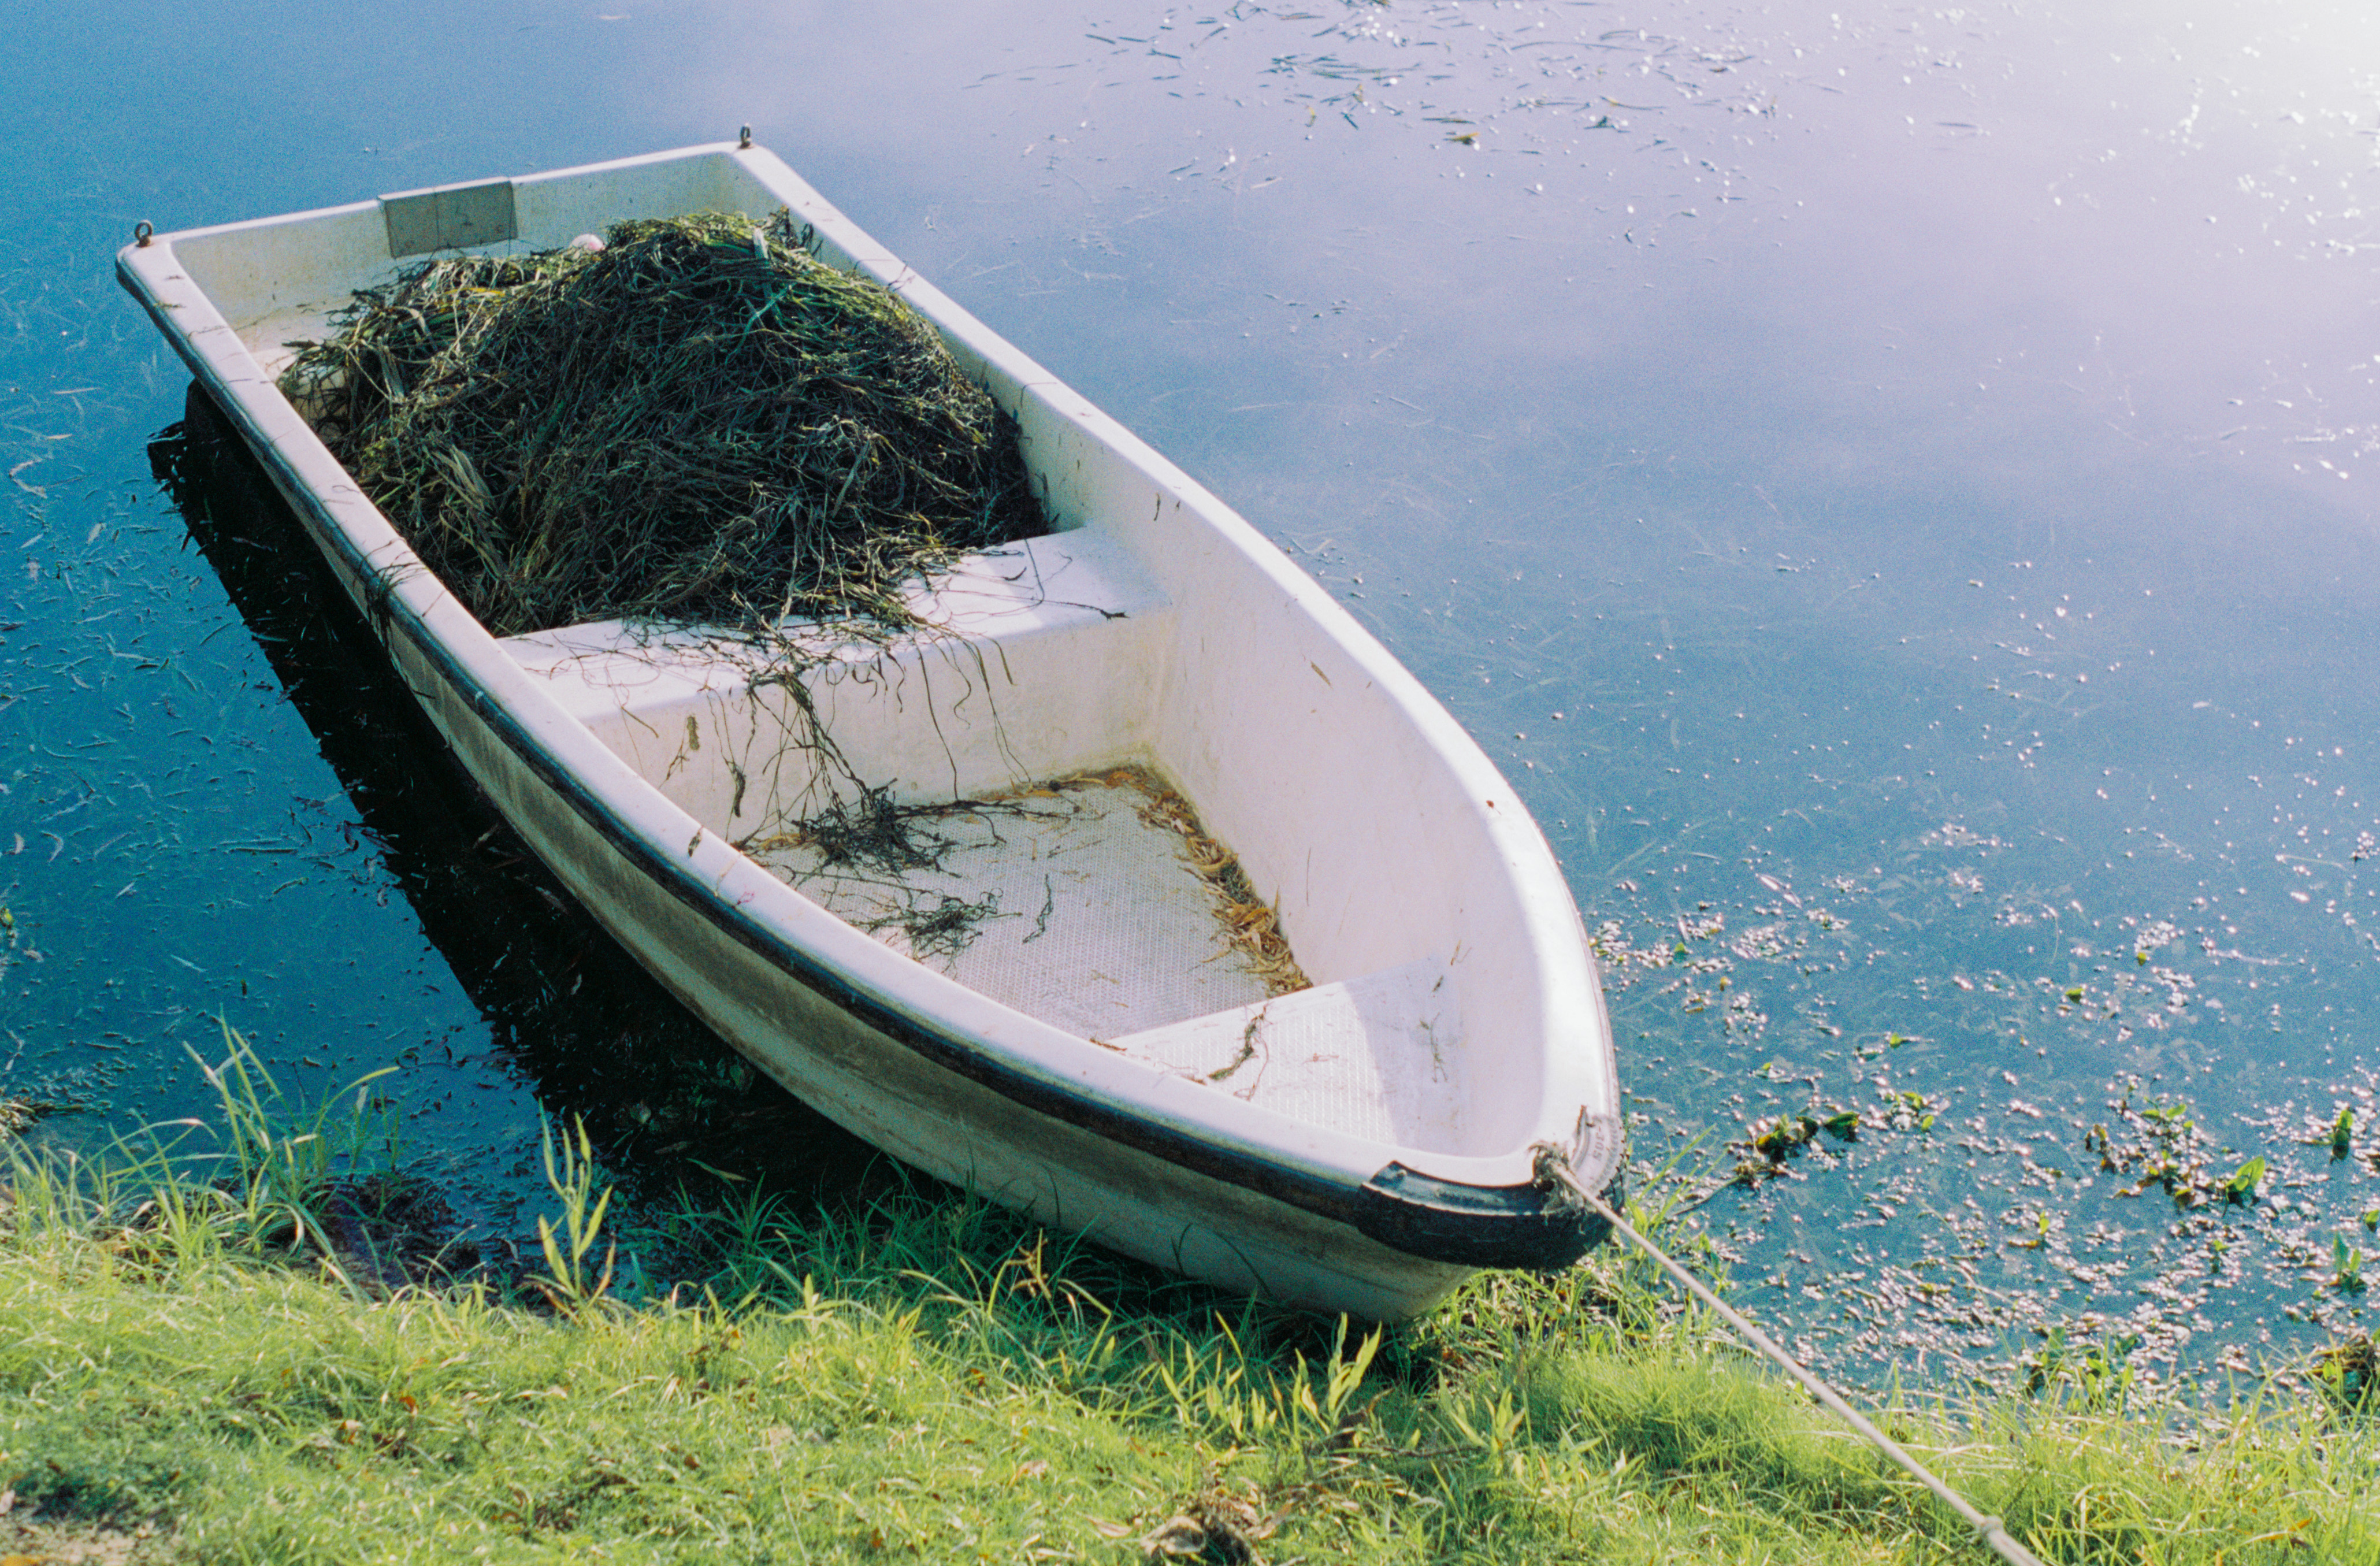
\includegraphics[width=0.45\textwidth]{Images/Photos/h5.jpg}
    }
\end{figure}



\begin{figure}[H]
    \centering

    \subfigure[白猫回眸]{
    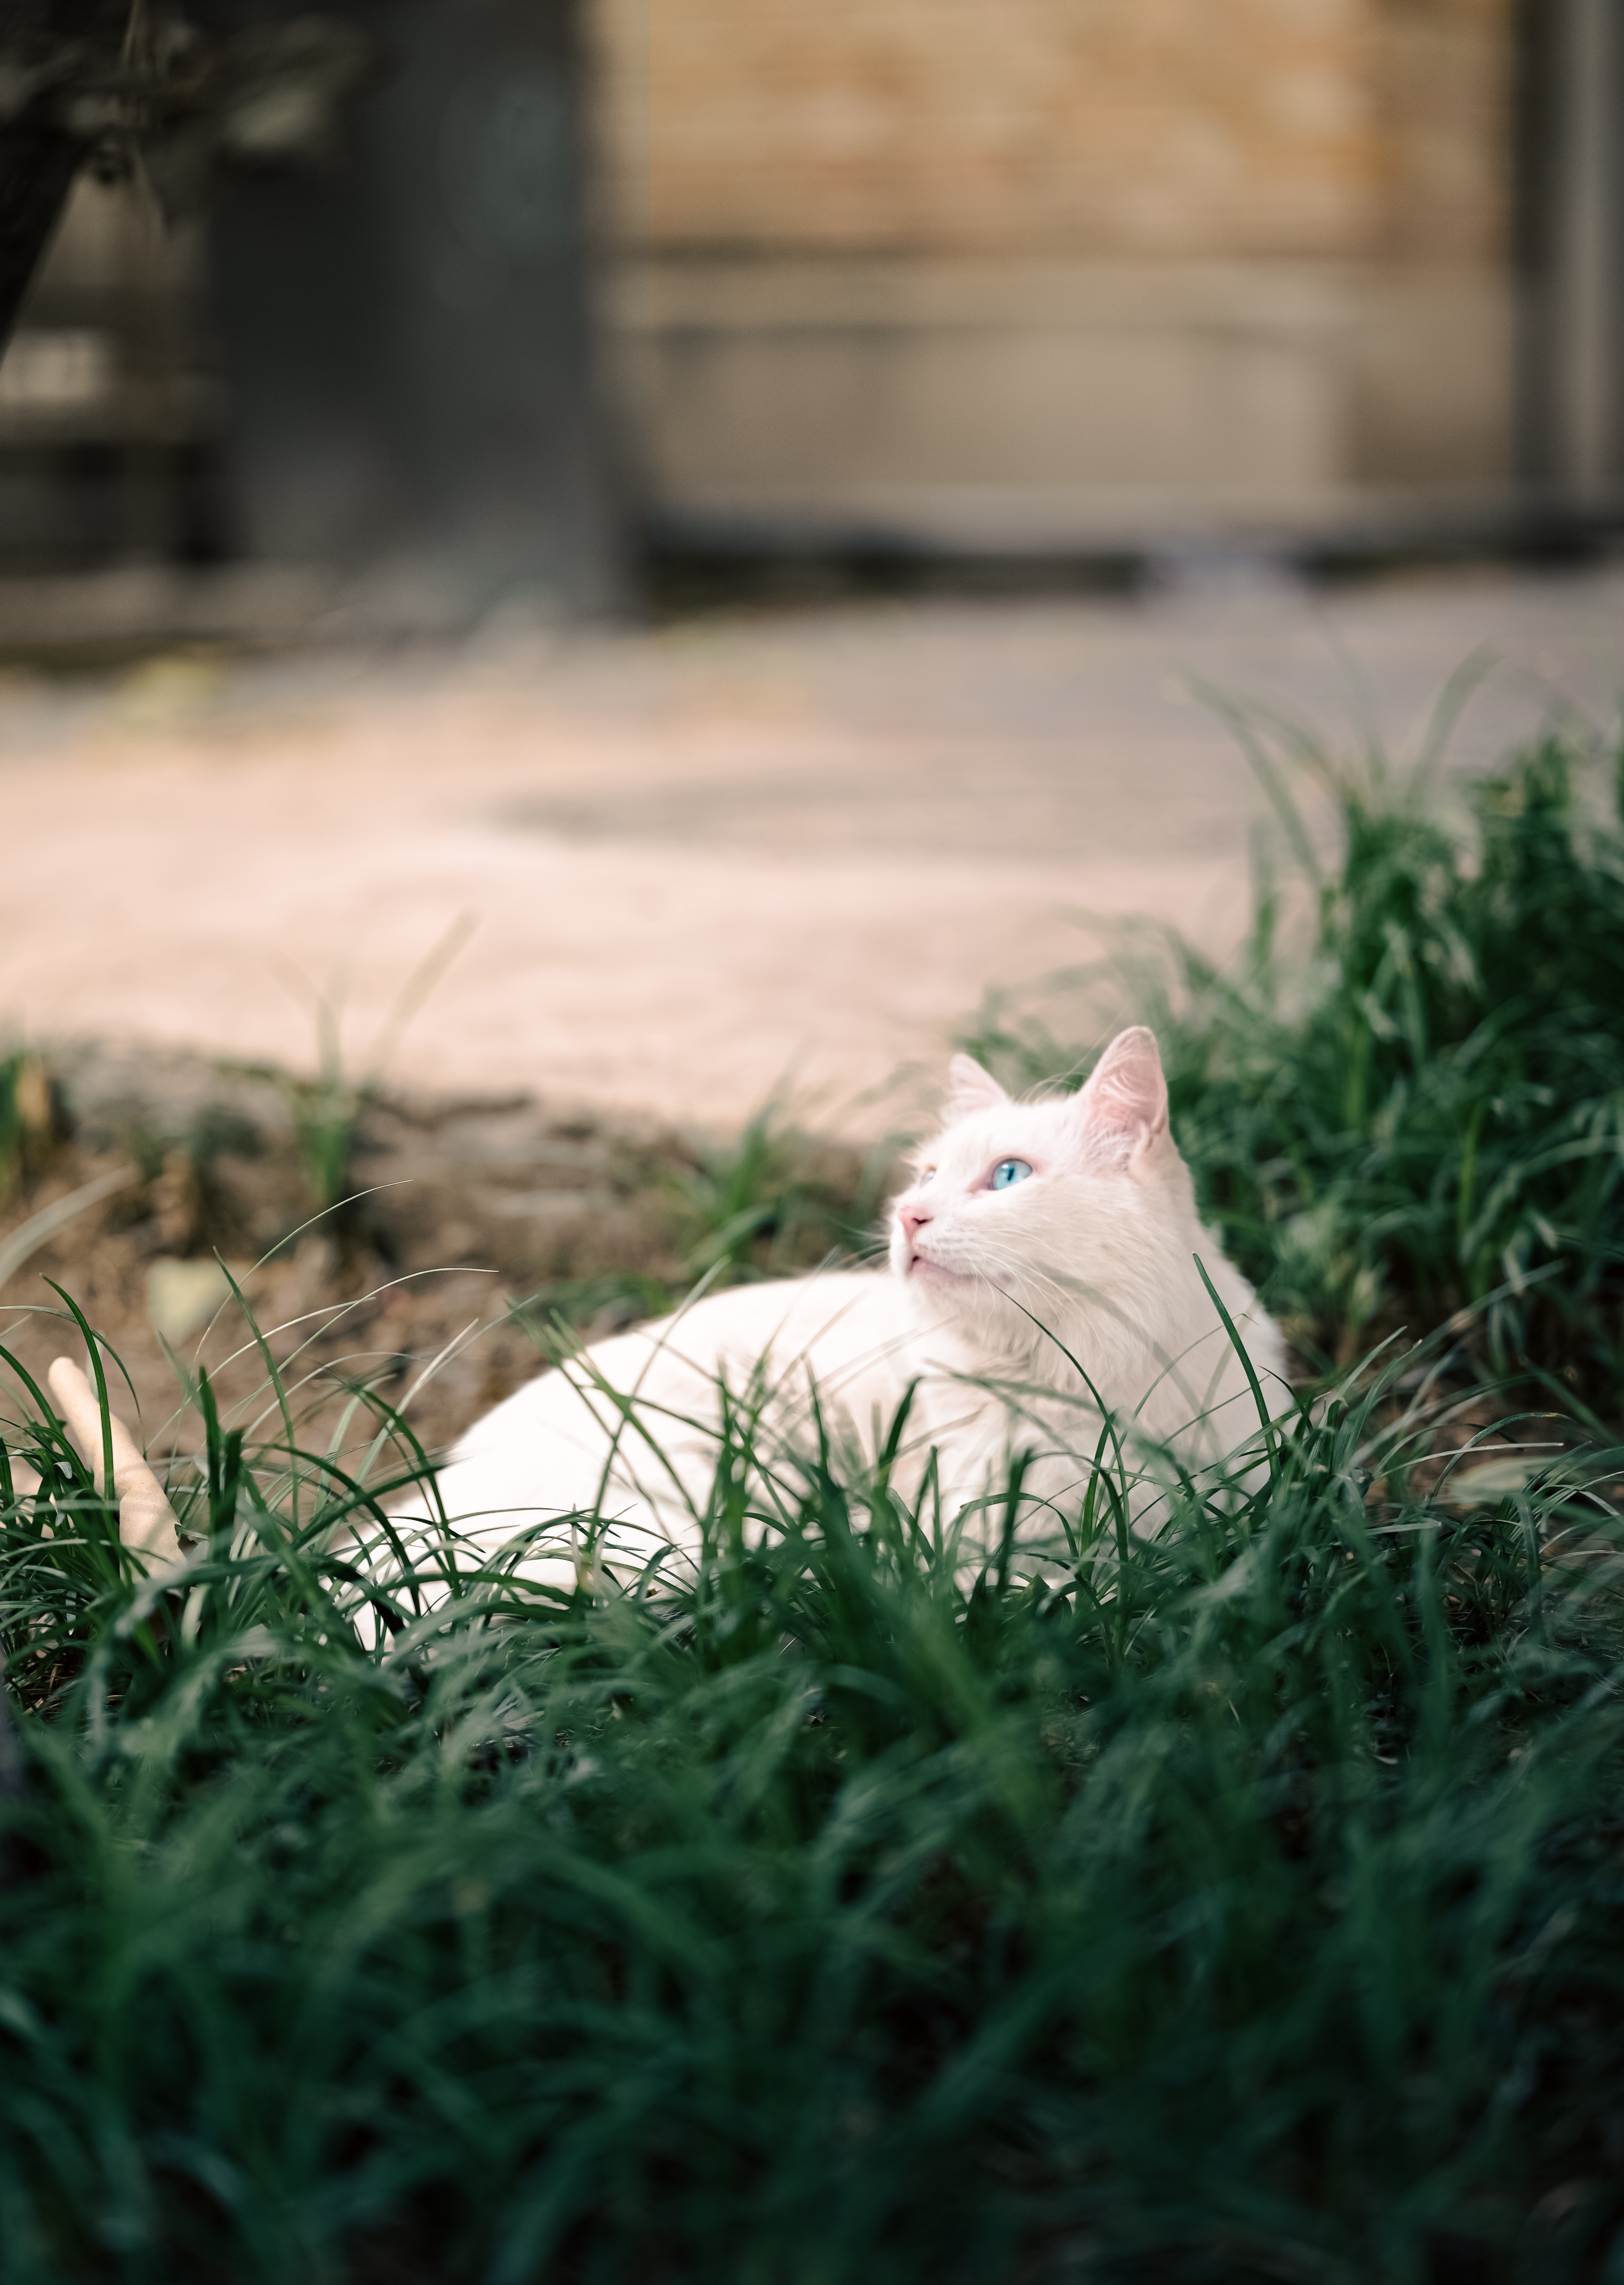
\includegraphics[width=0.45\textwidth]{Images/Photos/v3.jpg}}
    \subfigure[雨后水滴]{
    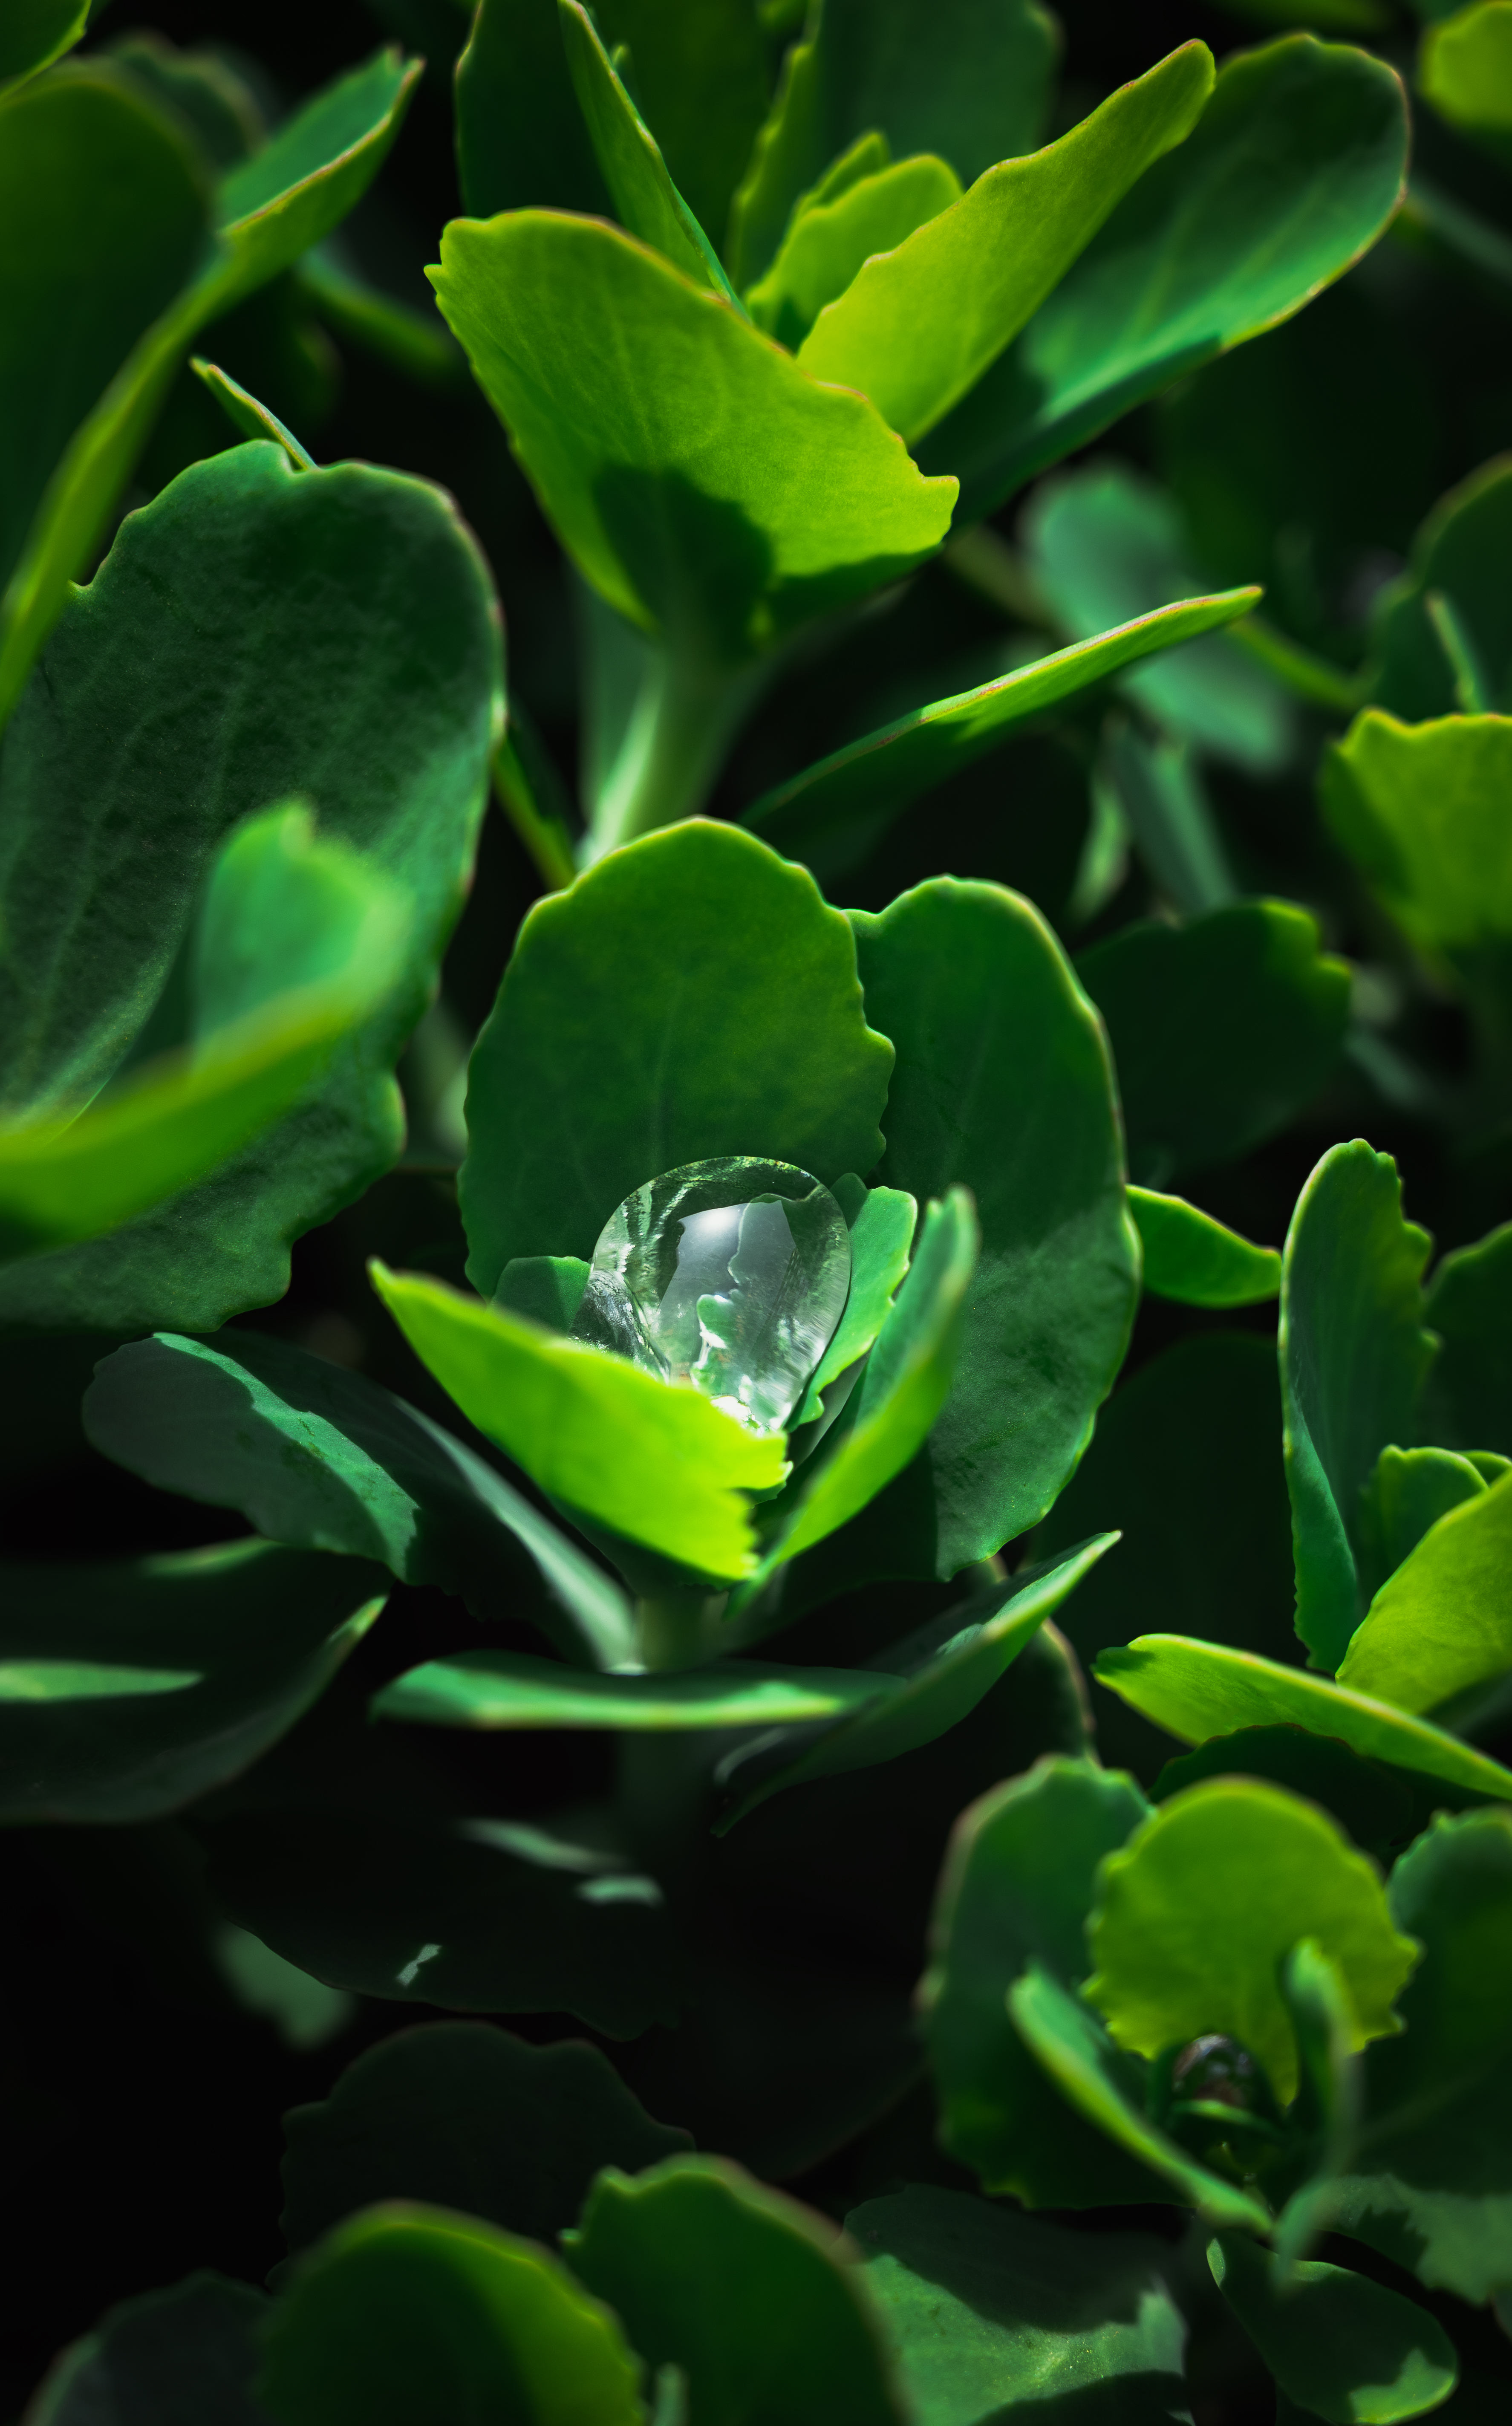
\includegraphics[width=0.45\textwidth]{Images/Photos/v2.jpg}}


    \subfigure[洞庭湖一角]{
    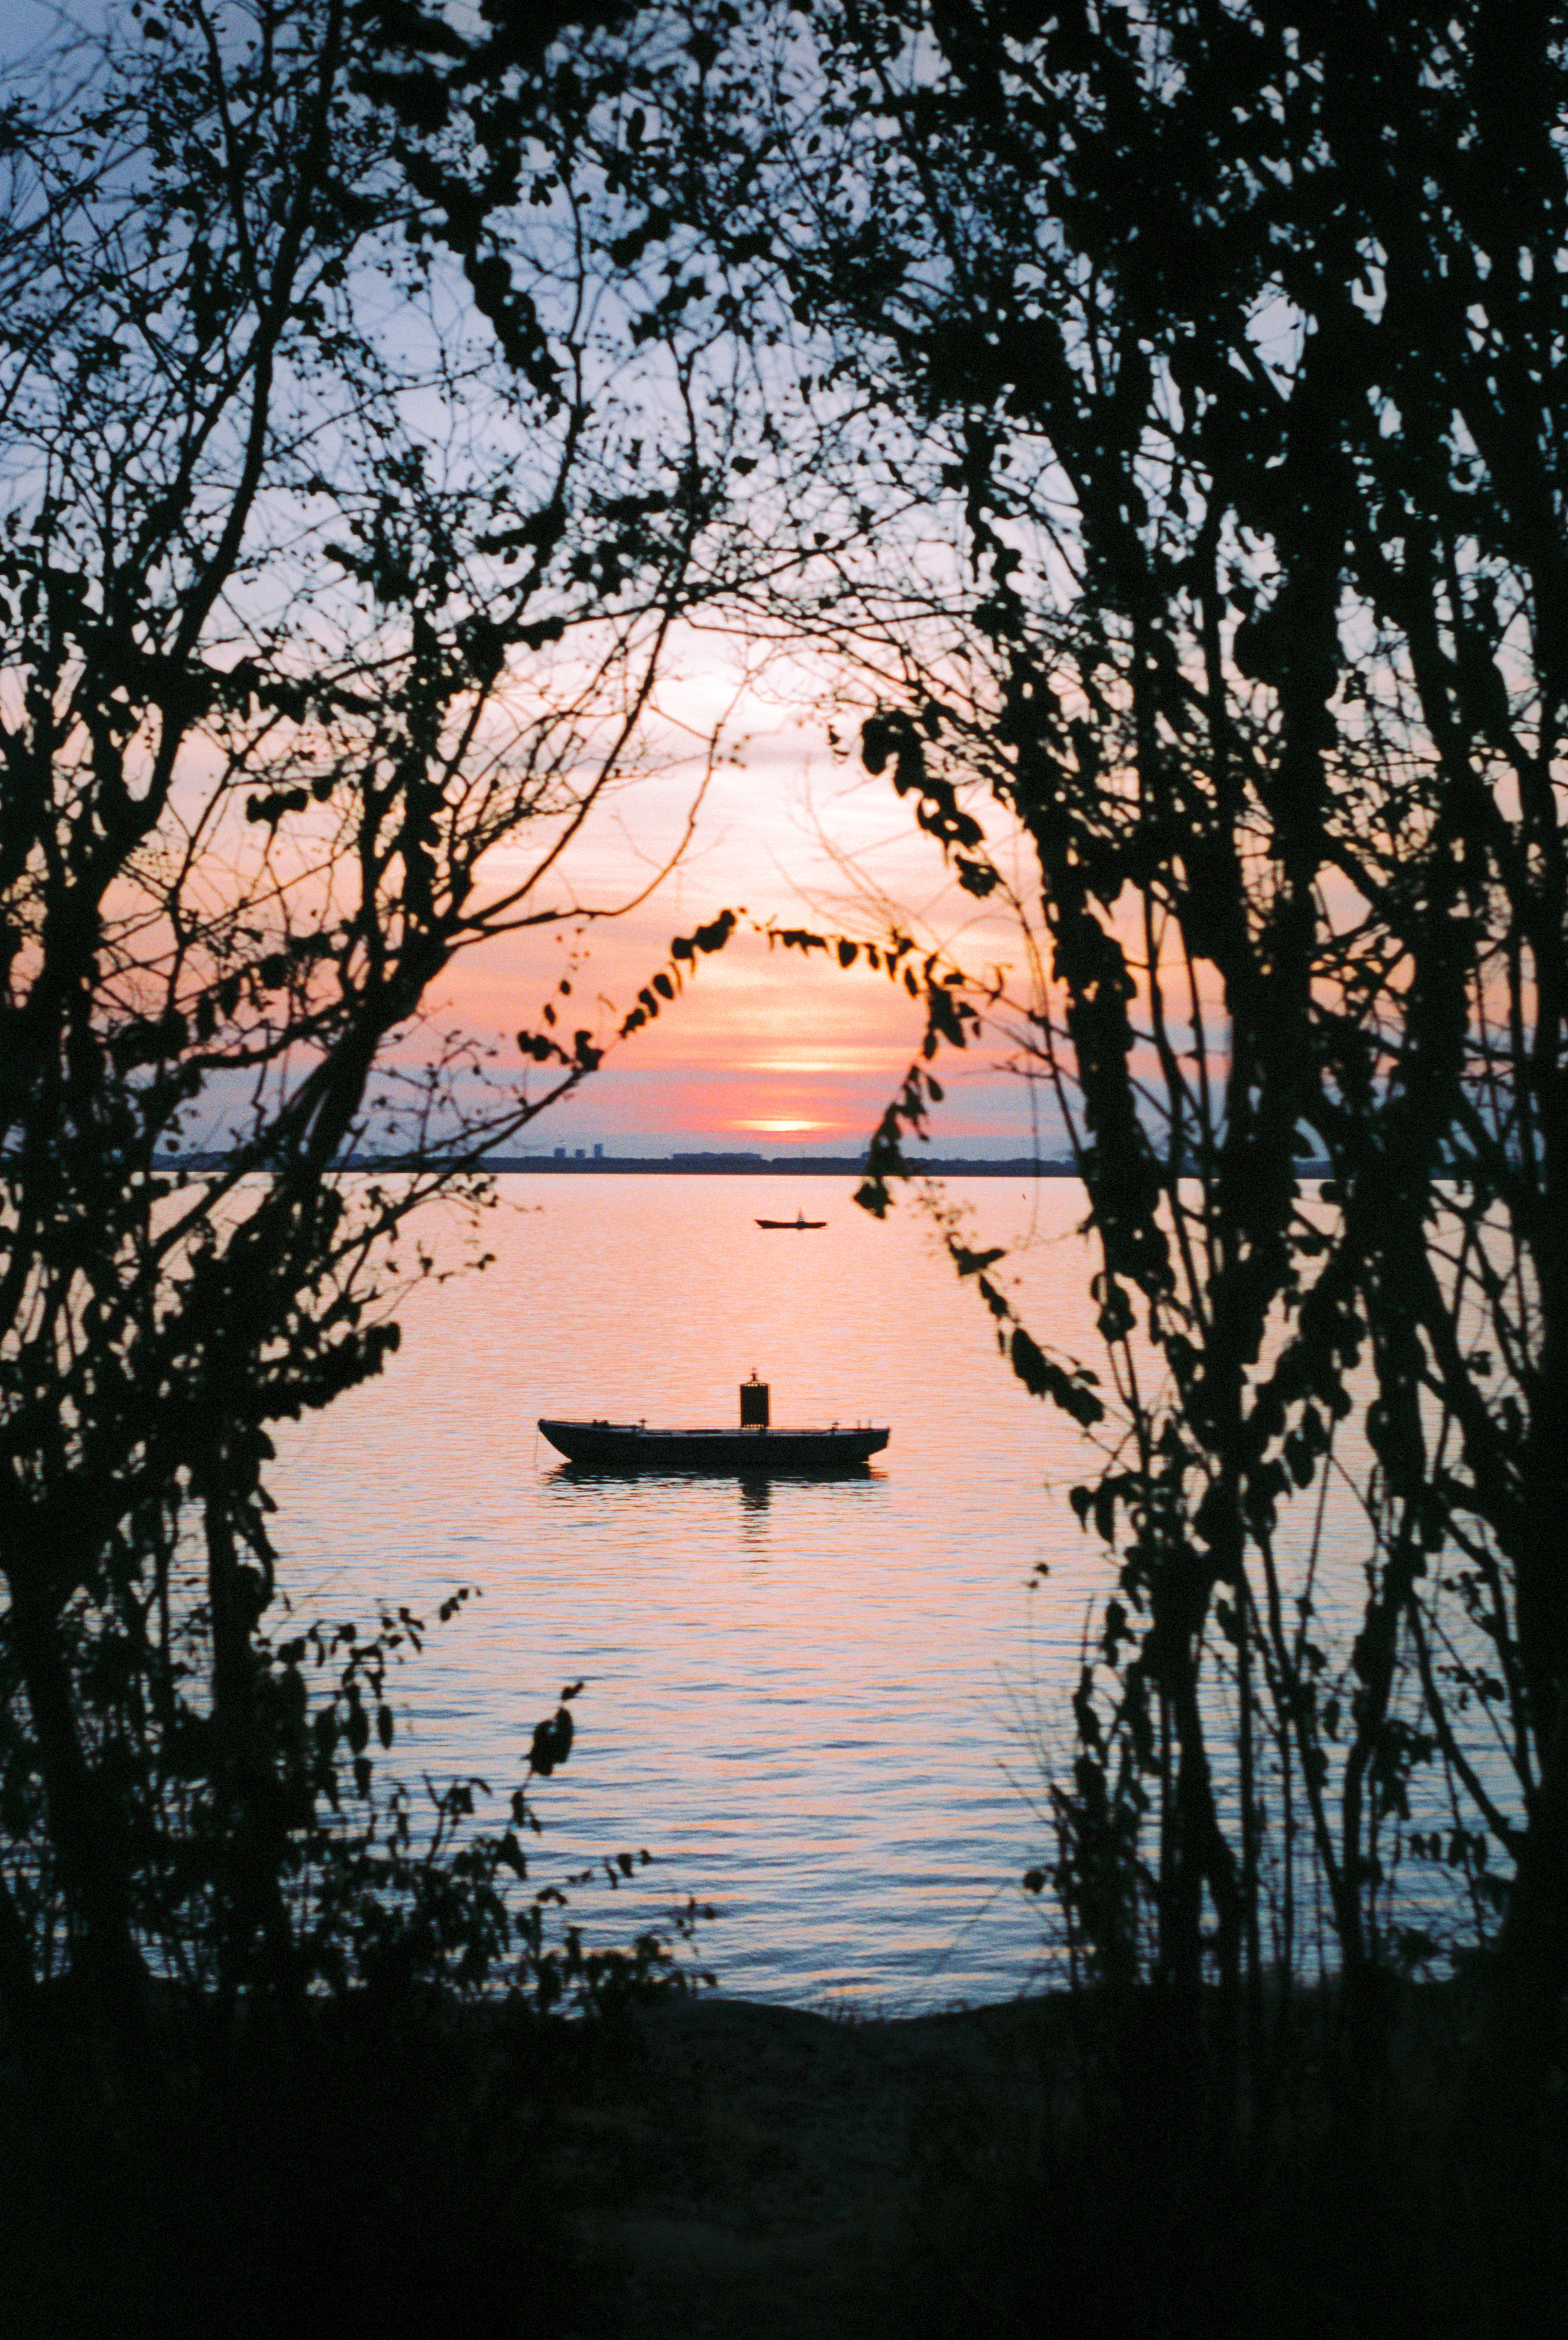
\includegraphics[width=0.45\textwidth]{Images/Photos/v1.jpg}}
    \subfigure[黄猫瞪眼]{
    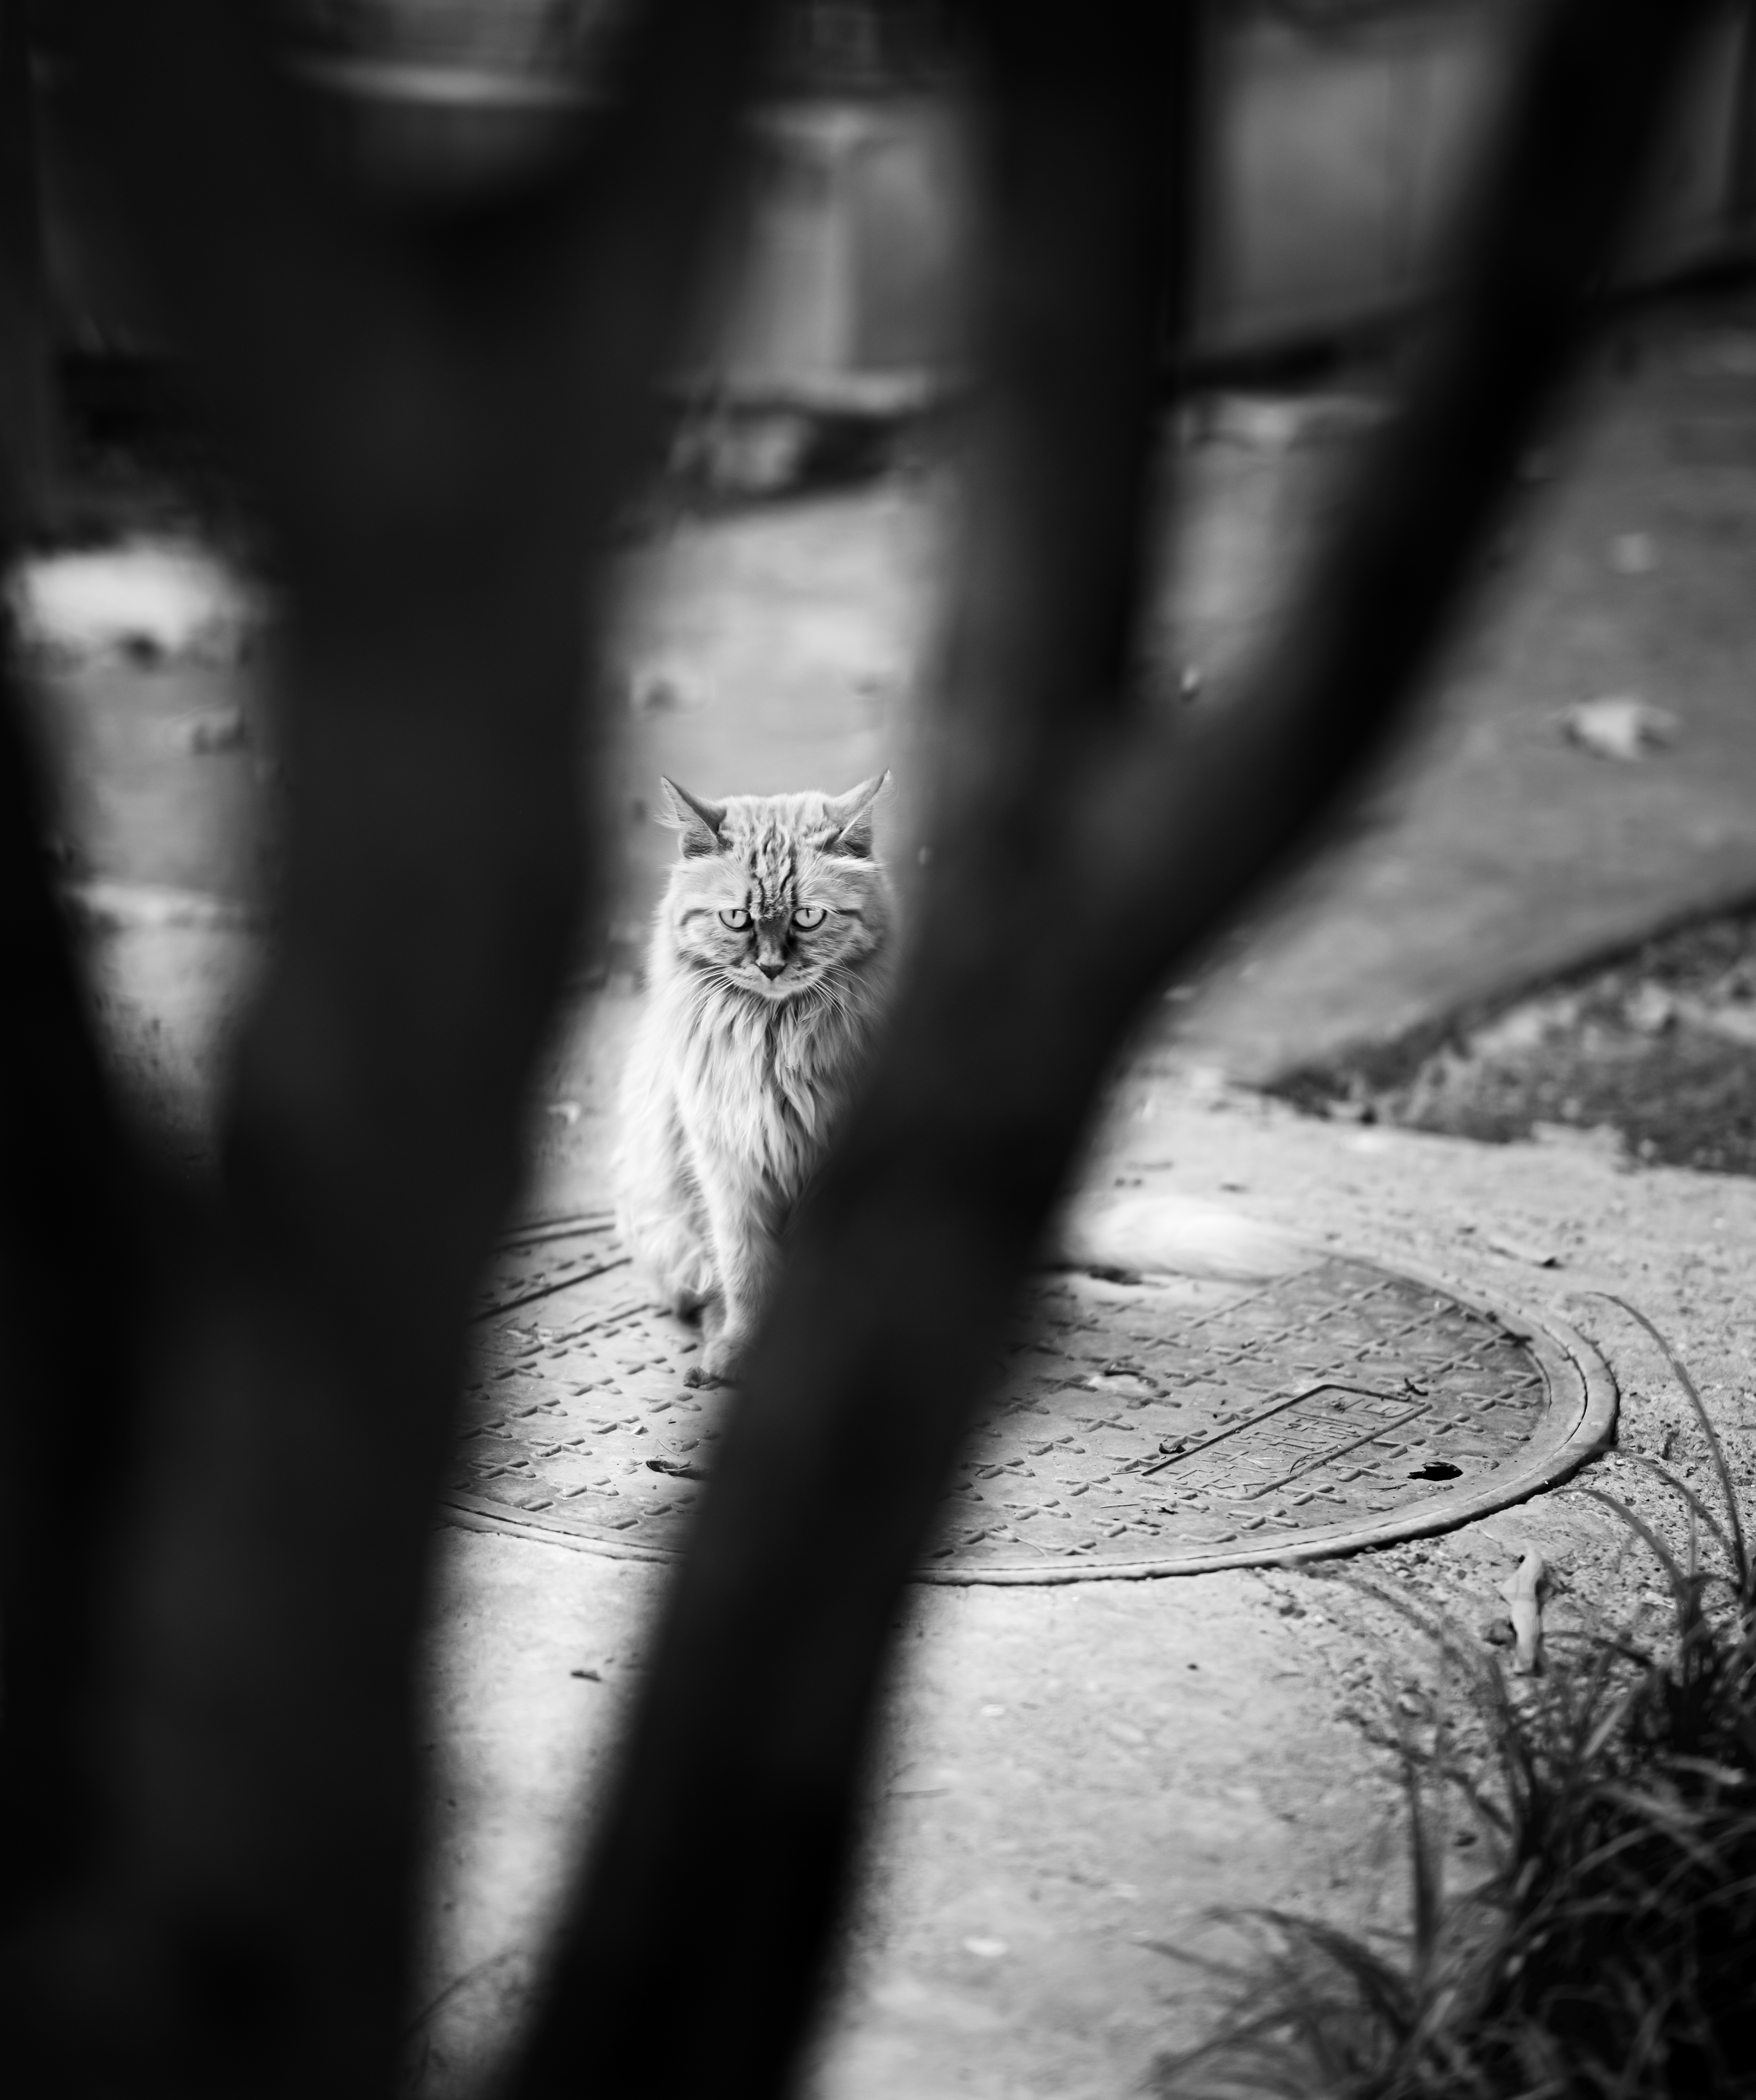
\includegraphics[width=0.45\textwidth]{Images/Photos/v4}}
\end{figure}